\documentclass[12pt,oneside,svgnames]{memoir}
\usepackage[italian]{babel} % language italian
\usepackage[T1]{fontenc}
\usepackage{lmodern}
\usepackage{amssymb,amsmath}
\usepackage{ifxetex,ifluatex}
\usepackage{fixltx2e} % provides \textsubscript
% to include cover page
\usepackage{pdfpages}
% use upquote if available, for straight quotes in verbatim environments
\IfFileExists{upquote.sty}{\usepackage{upquote}}{}
\ifnum 0\ifxetex 1\fi\ifluatex 1\fi=0 % if pdftex
  \usepackage[utf8]{inputenc}
\else % if luatex or xelatex
  \ifxetex
    \usepackage{mathspec}
    \usepackage{xltxtra,xunicode}
  \else
    \usepackage{fontspec}
  \fi
  \defaultfontfeatures{Mapping=tex-text,Scale=MatchLowercase}
  \newcommand{\euro}{€}
\fi
% use microtype if available
\IfFileExists{microtype.sty}{\usepackage{microtype}}{}
\usepackage[margin=1.2in]{geometry}
\usepackage{graphicx}
% Redefine \includegraphics so that, unless explicit options are
% given, the image width will not exceed the width of the page.
% Images get their normal width if they fit onto the page, but
% are scaled down if they would overflow the margins.
\makeatletter
\def\ScaleIfNeeded{%
  \ifdim\Gin@nat@width>\linewidth
    \linewidth
  \else
    \Gin@nat@width
  \fi
}
\makeatother
\let\Oldincludegraphics\includegraphics
{%
 \catcode`\@=11\relax%
 \gdef\includegraphics{\@ifnextchar[{\Oldincludegraphics}{\Oldincludegraphics[width=\ScaleIfNeeded]}}%
}%
\ifxetex
  \usepackage[setpagesize=false, % page size defined by xetex
              unicode=false, % unicode breaks when used with xetex
              xetex]{hyperref}
\else
  \usepackage[unicode=true]{hyperref}
\fi
\hypersetup{breaklinks=true,
            bookmarks=true,
            pdfauthor={},
            pdftitle={},
            colorlinks=true,
            citecolor=blue,
            urlcolor=blue,
            linkcolor=magenta,
            pdfborder={0 0 0}}
\urlstyle{same}  % don't use monospace font for urls
%\setlength{\parindent}{5pt}
%\setlength{\parskip}{6pt plus 2pt minus 1pt}
\setlength{\emergencystretch}{3em}  % prevent overfull lines
\setcounter{secnumdepth}{5}
\usepackage{xcolor}
%theme color
%\definecolor{maincolor}{RGB}{220, 22, 6} %CRIMSON
\definecolor{maincolor}{HTML}{2E6AB3}
%\definecolor{maincolor}{RGB}{70, 61, 140} %DARK SLATE BLUE
\usepackage{framed}
\usepackage{soul}
\definecolor{Light}{gray}{.90}
\sethlcolor{Light}
\newenvironment{quotationb}%
{\color{maincolor}\begin{leftbar}\begin{quotation}}%
{\end{quotation}\end{leftbar}\ignorespacesafterend}
% {\color{white}\begin{shaded}\begin{quotation}}%
% {\end{quotation}\end{shaded}\ignorespacesafterend}
\let\OldTexttt\texttt
\renewcommand{\texttt}[1]{\OldTexttt{\hl{#1}}}
\usepackage{tikz}

%define new chapter style (just for a nicer look)
\makechapterstyle{mystyle}{%
  \chapterstyle{default}
  \renewcommand*{\chapnumfont}{\normalfont\Huge\sffamily\bfseries}
  \renewcommand*{\chaptitlefont}{\normalfont\huge\sffamily\itshape\color{maincolor}}
  \settowidth{\chapindent}{\chapnumfont 111}
  \renewcommand*{\chapterheadstart}{}
  \renewcommand*{\chapnamefont}{\hfill\color{maincolor}\normalfont\Huge\sffamily\bfseries}
  \renewcommand*{\printchapternum}{%
  \begin{tikzpicture}[baseline={([yshift=-.6ex]current bounding box.center)}]
  \node[fill=maincolor,circle,text=white] {\thechapter};
  \end{tikzpicture}\\[1ex]
  \hrule height 1.5pt}
  \renewcommand*{\printchaptertitle}[1]{%
    {\chaptitlefont ##1}}
}

%use new chapter style
\chapterstyle{mystyle}

\author{}
\date{}

\begin{document}

\includepdf{src/content/frontcover/frontcover.pdf}
\addtocounter{page}{-1} % Do not count front cover as page
% Add empty page, not counted in page increment
\null
\thispagestyle{empty}%
\addtocounter{page}{-1}%
\newpage

{
\hypersetup{linkcolor=black}
\setcounter{tocdepth}{2}
\tableofcontents
}
\chapter{Introduzione}\label{introduzione}

\parskip0pt\parsep0pt

L'adozione internazionale è uno dei modi con i quali l'Italia si impegna
a garantire una famiglia adottiva ai minori che, in molti paesi del
mondo, non hanno la possibilità di crescere in un ambiente familiare
adeguato a dare loro l'assistenza morale e materiale di cui necessitano.
Crescere all'interno della propria famiglia biologica, per quanto
preferibile, infatti, non è sempre possibile (Scarpati 2012, 201) e
l'adozione è uno degli istituti che permettono di soddisfare il diritto
di ogni ``fanciullo'' (così come vengono definiti i bambini, le bambine,
i e le adolescenti nella traduzione italiana della \emph{Convention on
the Rights of the Child}) di avere una famiglia.

Quello dell'adozione è un istituto presente sin dall'antichità, basti
pensare alle figure storiche di Mosè o di Bruto, entrambi figli
adottivi. Esso però ha notevolmente cambiato il proprio significato
intrinseco nel corso del tempo: in Italia solo negli anni `80 lo sguardo
sull'adozione è stato ridefinito in funzione del minore e non
dell'adulto, ponendo alla base il diritto del primo ad avere una stabile
coppia di genitori e non quello della coppia di avere un figlio
(Scarpati 2012, 204).

Se l'adozione nazionale ha origini che si perdono nella storia antica,
quella di tipo internazionale ha un percorso piuttosto recente. L'inizio
del fenomeno si può infatti far risalire alla seconda guerra mondiale,
quando molte famiglie decisero di prendersi cura dei bambini e delle
bambine rimasti orfani nei diversi paesi coinvolti nel conflitto. Da
fenomeno legato alla logica della guerra, però, si diffuse largamente
tra le famiglie desiderose di un figlio, dal momento che gli orfanotrofi
nazionali non bastavano più a rispondere alla crescente richiesta delle
coppie di diventare genitori adottivi (\emph{Ivi}, 206).

Alla veloce diffusione dell'adozione internazionale non corrispose però
un'altrettanto veloce regolazione giuridica delle procedure adottive. Si
dovette aspettare il 1988 perché l'Ufficio permanente della Conferenza
dell'Aja di diritto internazionale privato iniziasse i lavori
preparatori (che durarono cinque anni), per redigere la
\emph{Convenzione per la tutela dei minori e la cooperazione in materia
di adozione internazionale} (\emph{Ibidem}). In essa, sin dal suo
preambolo, è chiarita la finalità principale dell'istituto adottivo:
``dare una famiglia permanente a quei minori per i quali non può essere
trovata una famiglia idonea nel loro Stato di origine'', per garantire
loro ``lo sviluppo armonioso della {[}\ldots{}{]} personalità'',
nell'interesse superiore di ogni Under18 e nel rispetto dei suoi diritti
fondamentali (\emph{Hague Adoption Convention} 1993, Preambolo).

Da allora sono stati raccolti molti dati e svolti diversi molti
multidisciplinari rispetto al fenomeno delle adozioni, sia a livello
quantitativo (ogni anno la Commissione per le adozioni internazionali,
con la collaborazione dell'Istituto degli Innocenti, redigono un
rapporto contenente dati e prospettive sulle adozioni internazionali in
Italia), sia di tipo qualitativo (cfr. Collana Studi e Ricerche della
Commissione per le adozioni internazionali \footnote{http://www.commissioneadozioni.it/it/bibliografia/studi-e-ricerche.aspx?UID=};
Lorenzini, Mancini 2007), oltre che diversi studi psicologici e
pedagogici. Appare dunque estesa la letteratura reperibile in materia,
ma gli enti che se ne occupano hanno rilevato una grossa lacuna relativa
ad un aspetto più specifico dell'adozione: vi è infatti un numero
estremamente limitato di ricerche italiane sul tema delle seconde
adozioni.

Con il termine ``seconda adozione'' si indica il percorso di quelle
famiglie che decidono di intraprendere una seconda volta l'iter adottivo
dopo averne già concluso un primo, desiderando dunque arricchirsi del
valore di un secondo figlio, ma dovendo allo stesso tempo andare in
contro ad una ristrutturazione di quegli equilibri interni al nucleo,
creati nella convivenza con il primo. Si tratta di un processo molto
delicato, al pari e se possibile ancor più della prima adozione, dal
momento che a dover essere costruito non è più soltanto un legame
filiale, ma anche un legame fraterno ``spesso tra bambini o bambine che
provengono da contesti di vita molto diversi'' (Franchetti et al. 2009,
282).

È necessario che le coppie prefigurino le possibili reazioni del
primogenito, il quale dovrebbe essere coinvolto adeguatamente nel
percorso e giungere preparato al primo incntro con il fratellino o la
sorellina. Coinvolgimento e preparazione del primogenito dovrebbero
avvenire però in modo delicato, graduale e facendo in modo che il
bambino o la bambina non sentano di sostenere il peso di un ruolo in
questa scelta che in realtà riguarda una decisione esclusivamente
propria dei genitori.

È importante, inoltre, tenere in considerazione la personale
rielaborazione emotiva del primo figlio o prima figlia, riguardo un
evento, come quello del viaggio nel paese di origine del
fratello/sorella, potenzialmente rievocativo di esperienze passate.
Questo secondo percorso, infatti, potrà in parte dar modo al primogenito
di rispondere ad alcuni dubbi e chiarire alcuni aspetti della propria
storia, dare ad essa una concretezza prima solo immaginata, ma in parte
susciterà anche il subentrare di molte altre domande.

I genitori peraltro, nel corso di questo secondo percorso adottivo,
devono fare i conti con la propria capacità di mettere in relazione i
sentimenti di tutela nei confronti del primo figlio con la disponibilità
di accoglienza del secondo, due aspetti difficili da fare conciliare
sina dalla preparazione dei documenti (per esempio relativamente alle
disponibilità sanitarie), e in seguito nel viaggio e nel percorso
post-adottivo.

Queste sono solo alcune delle numerose complessità che una famiglia con
due bambini adottati deve prepararsi ad affrontare; pertanto risulta
evidente che l'articolazione del fenomeno necessiti di studi
interdisciplinari approfonditi. In questa sede desidero dunque proporre
i risultati di una ricerca sociologica di tipo qualitativo svolta con lo
specifico obiettivo di dare rappresentazione, per quanto parziale, ad
una simile complessità.

Prima di entrare nei dettagli della ricerca desidero però proporre di
seguito un veloce excursus riguardo alcuni articoli della
\emph{Convenzione sui diritti dell'infanzia e dell'adolescenza }che,
oltre a permettere di introdurre meglio il lettore al tema qui
approfondito, si pongono in questo studio come speciali lenti o filtri
attraverso i quali leggere e analizzare il fenomeno delle seconde
adozioni.

\chapter{Children's rights lenses}\label{childrens-rights-lenses}

L'articolo 3 comma 1 della\href{http://www.unicef.org/crc/}{Convention
on the Rights of the Child} recita:

\emph{``In tutte le decisioni relative ai fanciulli, di competenza delle
istituzioni pubbliche o private di assistenza sociale, dei tribunali,
delle autorità amministrative o degli organi legislativi, l'interesse
superiore del fanciullo deve essere una considerazione preminente.''}

\emph{(CRC Art. 3, comma 1)}

Il ``\emph{best interest of the child}'' è dunque posto come ``valore
supremo'', da porre alla base di qualsiasi decisione relativa ad un
minore (Scarpati 2012, 105). Ma quale sia il migliore interesse, per
ogni \emph{Under18}, in ogni specifica situazione, in ogni contesto
sociale, politico, culturale, geografico e familiare non è assolutamente
questione di facile definizione. Occorre infatti tenere sempre a mente
il fatto che l'interesse da prendere in considerazione non è qualcosa di
generale e universale, bensì un interesse specifico di ciascun bambino,
bambina, ragazzo, ragazza (Scarpati 2012, 106).

Questo articolo è da porre dunque come filtro interpretativo di tutta la
Convenzione sui Diritti dell'Infanzia e dell'Adolescenza. Alla luce di
questo, pertanto, gli articoli analizzati di seguito, relativamente al
tema qui approfondito delle seconde adozioni, cui sono applicati, sono
stati in primis osservati tenendo ben a mente il fatto che, nel nostro
caso, il miglior interesse riguardi almeno due minori: il primo
figlio/figlia adottivo/a e il secondo o la seconda. È necessario dunque
prendere in considerazione e analizzare l'interazione che si crea tra i
diritti di entrambi i fanciulli: quali possono essere i \emph{best
interests} di ciascun singolo bambino/bambina e quali quelli dei due
fanciulli insieme?

\section{Diritto ad avere una famiglia (Artt. 9-20-21
CRC)}\label{diritto-ad-avere-una-famiglia-artt.-9-20-21-crc}

Quello di crescere all'interno di una famiglia, possibilmente quella
biologica, è diritto di ogni Under18. Se dunque i genitori biologici non
sono in grado di curare gli aspetti di assistenza affettiva e materiale
dei propri figli, la realtà pubblica deve innanzitutto attivarsi per
aiutarli a recuperare la propria adeguatezza.

Gli Stati parti vigilano affinché il fanciullo non sia separato dai suoi
genitori contro la loro volontà a meno che le autorità competenti non
decidano, sotto riserva di revisione giudiziaria e conformemente con le
leggi di procedura applicabili, che questa separazione è necessaria
nell'interesse preminente del fanciullo. Una decisione in questo senso
può essere necessaria in taluni casi particolari, ad esempio quando i
genitori maltrattino o trascurino il fanciullo, oppure se vivano
separati e una decisione debba essere presa riguardo al luogo di
residenza del fanciullo.

(CRC Art 9, comma 1)

Purtroppo però una minoranza non riesce ad adeguarsi, facendo permanere
il figlio in una situazione di abbandono morale e materiale.

\begin{enumerate}
\def\labelenumi{\arabic{enumi}.}
\item
  Ogni fanciullo il quale è temporaneamente o definitivamente privato
  del suo ambiente familiare oppure che non può essere lasciato in tale
  ambiente nel suo proprio interesse, ha diritto a una protezione e ad
  aiuti speciali dello Stato.
\item
  Gli Stati parti prevedono per questo fanciullo una protezione
  sostitutiva, in conformità con la loro legislazione nazionale.
\item
  Tale protezione sostitutiva può in particolare concretizzarsi per
  mezzo dell'affidamento familiare, della kafalah di diritto islamico,
  dell'adozione o, in caso di necessità, del collocamento in adeguati
  istituti per l'infanzia. Nell'effettuare una selezione tra queste
  soluzioni si terrà debitamente conto della necessità di una certa
  continuità nell'educazione del fanciullo, nonché della sua origine
  etnica, religiosa, culturale e linguistica.
\end{enumerate}

(CRC Art.20)

Solo nel momento in cui la famiglia viene dichiarata dall'autorità
giudiziaria quale ``abbandonica'', può dunque subentrare l'istituto
dell'adozione, in modo da poter dare al minorenne una famiglia adeguata.

Gli Stati parti che ammettono e/o autorizzano l'adozione si accertano
che l'interesse superiore del fanciullo sia la considerazione
fondamentale in materia e:

\begin{enumerate}
\def\labelenumi{\alph{enumi})}
\item
  vigilano affinché l'adozione di un fanciullo sia autorizzata solo
  dalle autorità competenti le quali verificano, in conformità con la
  legge e con le procedure applicabili e in base a tutte le informazioni
  affidabili relative al caso in esame, che l'adozione può essere
  effettuata in considerazione della situazione del bambino in rapporto
  al padre e alla madre, genitori e tutori legali e che, ove fosse
  necessario, le persone interessate hanno dato il loro consenso
  all'adozione in cognizione di causa, dopo aver acquisito i pareri
  necessari;
\item
  riconoscono che l'adozione all'estero può essere presa in
  considerazione come un altro mezzo per garantire le cure necessarie al
  fanciullo, qualora quest'ultimo non possa essere affidato a una
  famiglia affidataria o adottiva oppure essere allevato in maniera
  adeguata nel paese d'origine;
\item
  vigilano, in caso di adozione all'estero, affinché il fanciullo abbia
  il beneficio di garanzie e di norme equivalenti a quelle esistenti per
  le adozioni nazionali;
\item
  adottano ogni adeguata misura per vigilare affinché, in caso di
  adozione all'estero, il collocamento del fanciullo non diventi fonte
  di profitto materiale indebito per le persone che ne sono
  responsabili;
\item
  perseguono le finalità del presente articolo stipulando accordi o
  intese bilaterali o multilaterali a seconda dei casi, e si sforzano in
  questo contesto di vigilare affinché le sistemazioni di fanciulli
  all'estero siano effettuate dalle autorità o dagli organi competenti.
\end{enumerate}

(CRC Art. 21)

In particolare l'adozione di tipo internazionale entra in gioco per un
principio di sussidiarietà, caposaldo della \emph{Convenzione dell'Aja
per la tutela dei minori e la cooperazione in materia di adozione
internazionale} del 1993. Essa è quindi intesa sia come ``opportunità
genitoriale per un bambino'', che anche come ``forma di cooperazione
allo sviluppo, quando tutte le altre misure atte a garantire la
permanenza del bambino nel Paese d'origine siano risultate impossibili''
(Scarpati 2012, 212).

Nel caso delle seconde adozioni accade spesso che la famiglia adottiva
consideri la possibilità di dare questa opportunità genitoriale ad un
altro bambino o bambina per seguire il desiderio di far crescere il
primo figlio o figlia adottati con un fratellino o una sorellina.
Secondo i dati raccolti dalla CAI del 2013 (Commissione per le Adozioni
Internazionali 2013, 13), infatti, le motivazioni portate dalla famiglie
che vanno in contro ad una seconda adozione riguardano non tanto un
proprio desiderio di genitorialità, già soddisfatto con la prima
adozione, quanto una propria convinzione rispetto all'importanza delle
relazioni fraterne (Vedere Allegato 1 - Tavola Coppie adottive per
motivazione all'adozione (prima e seconda) - Anno 2013). Alla luce
dunque della convinzione che il ``miglior interesse''* *del proprio
figlio possa essere quello di avere un fratellino o una sorellina con
cui crescere, spesso le famiglie adottive decidono di procedere con una
seconda adozione. Assieme ad altri, proprio il tema delle motivazioni
che spingono i genitori adottivi ad intraprendere una seconda adozione
sarà oggetto di analisi di questo studio.

\section{Diritti di informazione, ascolto, espressione (Artt. 12-13
CRC)}\label{diritti-di-informazione-ascolto-espressione-artt.-12-13-crc}

Prima di procedere con il discorso più strettamente legato alla ricerca
sul tema delle seconde adozioni, desidero prendere in considerazione
ancora due articoli della CRC fondamentali per la realizzazione concreta
del \emph{best interest of the child.} Si tratta degli articoli 12 e 13
sul diritto del/della minorenne a partecipare alle scelte che lo/la
riguardano, in termini di informazione, ascolto ed espressione. Tenuta
conto della sua età e maturità l'\emph{Under18} ``capace di
discernimento'' deve, infatti, poter partecipare ai processi decisionali
che lo riguardano, esprimere la propria opinione, essere preso in
considerazione ed ascoltato (CRC Art.12 comma 1).

\begin{enumerate}
\def\labelenumi{\arabic{enumi}.}
\item
  Gli Stati parti garantiscono al fanciullo capace di discernimento il
  diritto di esprimere liberamente la sua opinione su ogni questione che
  lo interessa, le opinioni del fanciullo essendo debitamente prese in
  considerazione tenendo conto della sua età e del suo grado di
  maturità.
\item
  A tal fine, si darà in particolare al fanciullo la possibilità di
  essere ascoltato in ogni procedura giudiziaria o amministrativa che lo
  concerne, sia direttamente, sia tramite un rappresentante o un organo
  appropriato, in maniera compatibile con le regole di procedura della
  legislazione nazionale.
\end{enumerate}

(CRC Art. 12)

\begin{enumerate}
\def\labelenumi{\arabic{enumi}.}
\itemsep1pt\parskip0pt\parsep0pt
\item
  Il fanciullo ha diritto alla libertà di espressione. Questo diritto
  comprende la libertà di ricercare, di ricevere e di divulgare
  informazioni e idee di ogni specie, indipendentemente dalle frontiere,
  sotto forma orale, scritta, stampata o artistica, o con ogni altro
  mezzo a scelta del fanciullo.
\end{enumerate}

(CRC Art. 13 Comma 1)

All'interno del processo delle seconde adozioni questo diritto è da
declinare sia rispetto al minorenne che deve essere adottato/a, sia al
figlio/a già adottato. Il discorso si fa però particolarmente delicato
nel secondo caso, se si prendono in considerazione aspetti psicologici
che potrebbero coinvolgere il primogenito. Se apparentemente, infatti,
aver voce nella scelta di avere o meno un fratello o una sorella può
sembrare diritto applicato nel miglior interesse del bambino/a, in
realtà una simile responsabilità nella decisione di accogliere o meno un
nuovo membro della famiglia potrebbe avere conseguenze negative sul
piccolo/piccola.

Avere voce in capitolo, sostengono le psicologhe che tengono il corso
alle coppie in seconda adozione presso l'ente Cifa, significa che il
primogenito possa in seguito considerare l'opportunità di riportare il
proprio fratello o sorella nel paese d'origine o possa
auto-colpevolizzarsi qualora il rapporto tra i due sia conflittuale.
Considerare di aver preso la decisione sbagliata, acconsentendo
inizialmente all'arrivo di un secondogenito, può inoltre creare nel
primo o nella prima un conflitto interiore che impedisce di esternare i
propri sentimenti di eventuale malcontento.

Pertanto nel considerare la partecipazione del primo/a figlio/a rispetto
al secondo percorso adottivo, è necessario valutare molti aspetti, per
permettere il coinvolgimento opportuno, adatto all'età e alla
personalità di questo, e non responsabilizzante, in modo che venga
effettivamente messo in atto il migliore interesse di quel minore. Anche
su questo tema verterà una parte della ricerca, descritta nel seguente
capitolo.

\chapter{La ricerca: impostazione
metodologica}\label{la-ricerca-impostazione-metodologica}

CIFA è ad oggi il primo ente in Italia in termini di numero di adozioni
internazionali annuali; da più di trent'anni lavora quotidianamente per
creare ``legami di cuore'' tra figli e genitori non uniti da legami di
``sangue'' (CAI 2013, 5). Nel tempo l'associazione si è resa conto di
una forte carenza di studi nel contesto italiano in merito al fenomeno
ormai molto diffuso delle seconde adozioni.

Poiché si tratta di un argomento complesso, dalle ~``molteplici
sfaccettature'' (Franchetti et al. 2009, 274), ma soprattutto ancora
poco analizzato, si è vista la necessità di avviare una ricerca
qualitativa che non ha pretese di essere esaustiva del vasto argomento,
bensì desidera focalizzare l'attenzione su un piccolo campione che possa
far emergere motivazioni, aspettative, difficoltà, che caratterizzano la
complessità del secondo percorso adottivo.

L'obiettivo che Cifa si è posto con questo progetto, non è dunque quello
di colmare le lacune statistiche riguardo le seconde adozioni in Italia
(per perseguirlo sarebbe necessario uno studio quantitativo, oltre che
qualitativo, a livello nazionale), quanto piuttosto di fornire uno
sguardo in profondità che possa risultare una base qualitativa sulla
quale poter eventualmente costruire uno studio successivo di tipo
quantitativo. Ciò che qui interessa non è, pertanto, poter generalizzare
i dati raccolti, quanto comprendere dinamiche, emozioni, preoccupazioni
con le quali le famiglie decidono di intraprendere un secondo percorso
adottivo e il successo o meno del post-adozione, reso ancor più
complesso dalla relazione con un fratello o una sorella adottivi.

La rilevanza teorica di una ricerca su un tema poco studiato si
intreccia in questo caso con la rilevanza pragmatica
dell'approfondimento di un simile argomento. Quest'ultima è infatti
legata alla possibilità dell'ente di lavorare sulla procedura
pre-adottiva, la formazione delle famiglie che intraprendono questo
percorso, il loro accompagnamento nel viaggio e nel percorso
post-adottivo, in termini di miglioramento della qualità del servizio.

La domanda di ricerca che conduce il lavoro qui proposto si pone in
particolare l'obiettivo di far emergere quali possono essere, per le
famiglie che intraprendono una seconda adozione, i fattori problematici
e quelli protettivi dell'avere già un figlio adottato, le criticità e
gli aspetti positivi, in modo da poter studiare strategie per prevenire
o ridurre l'impatto delle prime e valorizzare i secondi. Inoltre, come
già detto, la ricerca si propone di avere una funzione ``prospettica''
per l'avvio di nuovi studi in merito.

\section{Il campione}\label{il-campione}

Il campione è costituito da diciotto coppie residenti in Piemonte e
Lombardia che hanno effettuato la loro seconda (o terza) adozione presso
CIFA. La scelta è avvenuta mediante un campionamento strategico, svolto
con l'aiuto dell'équipe psicologica dell'ente, al fine di coinvolgere le
famiglie che hanno presentato alcune peculiarità nel secondo iter
adottivo o problematicità rispetto al primo o al secondo percorso
post-adozione.

Il campione risulta abbastanza omogeneo per ciò che riguarda il capitale
sociale ed economico posseduto dai genitori (gli intervistati infatti
sono per la maggior parte diplomati o laureati, con reddito medio-alto),
mentre è disomogeneo rispetto all'età (dei genitori e dei figli), al
sesso dei bambini, alla loro provenienze e alla distanza tra la prima e
la seconda adozione.

Le famiglie selezionate non sono rappresentative della popolazione di
famiglie adottive per la seconda volta

\section{Le interviste}\label{le-interviste}

Le interviste hanno avuto luogo nella sede centrale CIFA a Torino e
presso lo sportello informativo di Milano e hanno previsto circa un'ora
di colloquio ad entrambi i membri della coppia, intervistati insieme.

La traccia (Allegato 2) è costituita da domande aperte relative alle
esperienze adottive della famiglia, nel tentativo di rilevare in parte
proponendo agli stessi genitori una riflessione di confronto tra i due
percorsi di adozione, in parte invece mediante domande meno dirette,
quali siano state le differenze tra la prima esperienza e la seconda, e
soprattutto quali i fattori protettivi e quali quelli critici di
un'adozione in presenza di un fratello o una sorella già adottato/a.
Sono state inoltre poste agli intervistati domande riguardanti la
valutazione della propria situazione, desideri, aspettative, rimorsi,
speranze e delusioni.

Tutte le interviste sono state registrate e poi trascritte, diventando
testi da esplorare, analizzare, indagare, nella scelta delle parole,
nelle espressioni, nell'uso del linguaggio, delle coloriture emotive,
nella posizione del locutore rispetto a ciò che esprime, nelle tracce di
conflitti interiori, pur nella consapevolezza che ciò che viene mostrato
all'intervistatore è filtrato da maschere goffmaniane che tendono a
proporre rappresentazioni di ciò che è ritenuto socialmente accettabile.
Ho costruito sinossi per ciascun nucleo familiare, integrate con i dati
raccolti precedentemente nei colloqui delle psicologhe che seguono le
coppie nel periodo post-adottivo, e creato apposite tabelle Excel di
raccolta dati, in modo da rendere più semplice la successiva fase di
analisi.

\section{Limiti e prospettive}\label{limiti-e-prospettive}

Per questioni logistiche è stato necessario limitare la ricerca allo
svolgimento di interviste ai genitori adottivi di un secondo figlio o
figlia, sul territorio di Piemonte e Lombardia, con ente Cifa.
Interessante sarebbe estendere la ricerca a coppie che hanno conferito
anche con altri enti, su tutto il territorio nazionale. Si potrebbe
inoltre pensare ad un coinvolgimento degli stessi figli adottati, in
particolare le prime adozioni, le cui età possano permettere lo
svolgimento di interviste, opportunamente costruite a misura di Under18.
Infine sarebbe opportuno impostare successive ricerche proponendo un
confronto tra i percorsi post-adottivi internazionali e nazionali, in
modo da comprendere se vi sia una discrepanza o meno nelle possibilità
di successo delle seconde adozioni.

Per ciò che concerne il metodo di raccolta dei dati, l'intervista
potrebbe comportare alcuni depistaggi e nascondimenti messi in atto
dalle coppie, la cui cooperazione nella ricerca della ``verità'' non è
da dare per scontata. Spesso infatti, a maggior ragione in un colloquio
relativo al successo o meno di un percorso post-adottivo, il goffmaniano
``salvare la faccia'', per condividere con l'intervistatore solo ciò che
si ritiene socialmente accettabile, rende lo statuto epistemico del
materiale empirico raccolto incerto e congetturale (Cardano 2011, 9).
Immaginando una disponibilità maggiore di tempo e risorse, potrebbe
essere interessante riproporre questo studio intervistando separatamente
i coniugi e ipotizzando un'intervista appositamente costruita, anche ai
figli, o immaginando uno strumento di rilevazione differente come per
esempio lo \emph{shadowing}. Il focus group invece mi è sembrata
un'ipotesi da scartare per la delicatezza del tema e la specificità di
ogni singolo caso in studio.

\chapter{La ricerca: analisi e
risultati}\label{la-ricerca-analisi-e-risultati}

In questo capitolo desidero presentare i risultati della ricerca, emersi
dall'analisi delle interviste, ripercorrendo tutti gli argomenti di
interesse, come pennellate che nel loro insieme forniranno al lettore un
dipinto articolato e a tratti non ben definito di una tematica difficile
da cogliere nella sua complessità, come quella delle seconde adozioni.

Ho deciso di procedere in modo temporale, affrontando dapprima le
tematiche relative al percorso precedente la seconda adozione, quali le
motivazioni alla base della scelta di intraprendere un secondo percorso
adottivo, le aspettative riposte in questo, le complessità prefigurate
dai genitori, il ruolo della rete di sostegno parentale e amicale in
questa fase, insieme a tutti quegli aspetti che riguardano la mediazione
tra la tutela del proprio figlio o figlia e la disponibilità
nell'accoglienza del secondo o seconda (par. 4.1).

In seguito ho focalizzato l'attenzione sul tema del viaggio, la
preparazione ad esso, le diverse modalità di coinvolgimento del
primogenito e la sua gestione emotiva rispetto alla possibilità di
ripercorrere un sentiero in qualche modo già vissuto, oltre che il suo
ruolo nell'accoglienza del fratellino/sorellina in famiglia (par 4.2).

Infine ho dedicato l'ultimo paragrafo di questo capitolo al periodo (per
alcune famiglie intervistate più breve, per altre più lungo) del
post-adozione, approfondendo in particolar modo la relazione tra i
fratelli, le complessità della conoscenza, del rispettivo
riconoscimento, i fattori protettivi e critici di questo rapporto ed il
ruolo dei genitori in questa fase (par. 4.3).

\section{Allargare la famiglia: aspettative e preoccupazioni di un
secondo percorso
adottivo}\label{allargare-la-famiglia-aspettative-e-preoccupazioni-di-un-secondo-percorso-adottivo}

\begin{quotationb}
``L'adozione rappresenta un po' il nostro modo di fare famiglia
{[}\ldots{}{]} e la seconda adozione ne è la riprova'' (Luigi Lava)
\end{quotationb}

afferma Luigi Lava nel corso dell'intervista, evidenziando la
naturalezza con cui lui e sua moglie si sono sentiti di affrontare un
secondo percorso adottivo, per dare completezza al proprio nucleo
familiare. In realtà la scelta di intraprendere questa strada è stata
per loro, come per quasi tutte le altre coppie del campione, costellata
di momenti di preoccupazione. In questo paragrafo, prenderò in
considerazione il periodo precedente l'incontro con il proprio secondo
figlio o figlia: dalla spinta motivazionale, alle aspettative,
focalizzando l'attenzione sulle criticità prefigurate.

Sin dall'analisi delle motivazioni riferite dagli intervistati emerge un
panorama non omogeneo: se tra le coppie in prima adozione la scelta di
intraprendere questa strada è riconducibile al desiderio di
genitorialità insoddisfatto dalla propria ``impossibilità di procreare''
(CAI 2013, 13), le motivazioni alla base di un secondo percorso adottivo
appaiono più differenziate. Spesso la spinta proviene dall'idea di un
modello familiare allargato (``Abbiamo sempre voluto una famiglia
numerosa'' \footnote{Cit. Bianca Bosco}, ``Non si cresce da figli
unici!'' \footnote{Cit. Francesca Fragola}), ma gli assunti su cui
questo poggia sono diversi da famiglia a famiglia. Dal desiderio di
sperimentare forme di genitorialità diverse, a quello di dare una
famiglia ad un altro bambino che non ce l'ha, dalla convinzione che
crescere in due possa essere più educativo in termini di condivisione di
giochi, spazi, tempo e affetto, all'idea che questo possa creare
maggiore sicurezza per la complicità con un pari:

\begin{quotationb}
Secondo me è molto importante avere qualcuno che non sia una mamma o un
papà a cui magari dire le cose, con cui avere una minima complicità e
soprattutto mi sembrava che nel loro caso, cioè già in un certo senso li
sradichi dal loro territorio, arrivano in un territorio nuovo, vero che
poi creano la famiglia, c'è la società che li accoglie, però comunque mi
sembrava che avessero bisogno anche di un altro punto di riferimento,
cioè proprio un essere sradicati e doversi trovare da soli,
completamente, a dover affrontare tutte le difficoltà che la vita ti può
riservare, per quanto ci siano i genitori, però secondo me avere un
fratello è una cosa diversa, è un punto di appoggio in più e secondo me
poteva servirgli insomma. (Milena Muschio)
\end{quotationb}

Pamela Pioppo spera che i propri figli possano ``ritrovarsi nella storia
dell'altro'' e anche la famiglia Risacca sostiene l'importanza della
relazione fraterna immaginandola proprio come possibilità di
condivisione di un'esperienza di vita simile:

\begin{quotationb}
Il pensiero che un fratello ha percorso un pezzo di strada uguale alla
tua magari può aiutarti. (Rachele Risacca)
\end{quotationb}

Gli elementi fondamentali che le famiglie prendono in considerazione per
decidere di avventurarsi in un nuovo percorso adottivo riguardano il
bilancio della prima adozione e la valutazione dell'inserimento di un
secondo figlio/a all'interno del nucleo (Franchetti et al. 2009, 281).
Spesso accade, pertanto, che la scelta di adottare un secondo figlio sia
presa sull'onda dell'ottimismo dovuto ad un primo percorso adottivo
molto positivo:

\begin{quotationb}
È stato talmente bello che abbiamo fatto la seconda! {[}\ldots{}{]} Noi
già subito pensavamo, no dobbiamo farne un'altra, subito, perché è stata
un'esperienza bella proprio. (Federica Foglia)
\end{quotationb}

\begin{quotationb}
Quando tu ce l'hai così belle (esperienze adottive come la prima) al di
là del fatto di voler magari avere una famiglia numerosa, noi abbiamo
fatto subito una seconda domanda. {[}\ldots{}{]} Aspettative altissime
come ente e come percorso con il bimbo. È andata veramente bene e quindi
si abbiamo subito pensato ``no no vogliamo la seconda''. (Rebecca
Resina)
\end{quotationb}

In questi casi le aspettative sono altissime e il rischio di
disattenderle altrettanto grande. Come sostengono le psicologhe del Cifa
nel corso formativo alle famiglie che intendono intraprendere un secondo
percorso adottivo, infatti, ogni adozione è a se stante, ogni esperienza
diversa e aspettative troppo grandi potrebbero essere deluse dalla
presenza di difficoltà non prefigurate. Il consiglio di Milena Muschio
ad altre famiglie in seconda adozione è infatti quello di:

\begin{quotationb}
partire un po' più come una tabula rasa, partire senza delle particolari
aspettative, però non andare prevenuto con l'ok, per il primo è stato
così per cui sarà così, cioè non avere delle aspettative uguali alla
prima adozione, cioè capire che veramente sono due percorsi che possono
essere completamente diversi. (Milena Muschio)
\end{quotationb}

Il successo del primo percorso non è indicatore del successo del
secondo, sia a livello puramente tecnico-burocratico (tempi di attesa,
abbinamento, viaggio), sia per il fatto che si tratta di un altro
bambino o bambina, con un'altra storia, un altro vissuto, un altro
carattere. Anche i genitori non si possono considerare più gli stessi,
essi sono infatti cambiati come coppia e nella proprie capacità
genitoriali.

Inoltre nel secondo percorso adottivo entrano in gioco fattori diversi,
primo tra i quali la relazione tra fratelli. Problemi, infatti, possono
sorgere sia per il secondogenito, in difficoltà a conquistarsi il
proprio spazio all'interno del nucleo familiare, sia per il primo, il
quale potrebbe per esempio reagire in modo negativo all'imposizione di
una divisione dell'affetto dei genitori con un altro bambino.
Quest'ultimo è il caso della famiglia Loto, la quale non aveva
considerato la possibilità che il primogenito potesse avere un
atteggiamento reattivo, che riverberasse sul rapporto col fratello e sul
rendimento scolastico:

\begin{quotationb}
Cioè noi non pensavamo che Lorenzo avrebbe avuto tutte queste
difficoltà, perché non c'erano i presupposti, alla scuola materna non
era mai emerso nulla di sospetto diciamo, lui è sempre stato un bambino
tranquillo e sereno, sorridente, noi non ci saremmo mai immaginati che
lui avrebbe avuto un'evoluzione di questo genere. (Luisa Loto)
\end{quotationb}

D'altra parte, al di là delle elevate aspettative da parte delle coppie,
una consapevolezza delle difficoltà che si sarebbero potute incontrare
era comunque presente nella maggior parte degli intervistati. Alcuni di
essi hanno confessato il proprio timore di intraprendere, come famiglia
e non più solo come coppia, un percorso così complesso e poco definito
come l'adozione di un bambino proveniente da un altro paese. La
preoccupazione condivisa dalla maggior parte del campione riguardava la
necessità di ricreare un nuovo equilibrio familiare, spesso trovato solo
da poco con il primogenito:

\begin{quotationb}
Della serie ``abbiamo trovato un equilibrio adesso? Adesso cambia
tutto'' (Pamela Pioppo)
\end{quotationb}

\begin{quotationb}
Quando abbiamo deciso di fare questa seconda adozione il dubbio era
sempre su questo bimbo che doveva arrivare, se questo bimbo avesse avuto
problemi, poteva appunto destabilizzare l'equilibrio che si era già
creato eccetera eccetera. (Luisa Loto)
\end{quotationb}

Per ciò che riguarda le preoccupazioni genitoriali (``Sarò in grado? Non
sarò in grado? Mi riconoscerà? Lo riconoscerò?'') il campione si colloca
su due estremi opposti: vi sono coppie che ritengono che il bagaglio di
esperienza costruito nel corso della prima adozione possa essere un
utile strumento di sostegno per affrontare la seconda\ldots{}

\begin{quotationb}
All'inizio diventi genitore per la prima volta e quindi non sai come
diventi come mamma, come papà, eeee sei sotto pressione sotto tutti i
punti di vista, invece dopo, è difficile perché magari devi valutare
ovviamente anche l'arrivo per il fratello, quindi come la prende, la
gelosia. Però sotto l'aspetto del divento mamma è un po' più semplice.
(Federica Foglia)
\end{quotationb}

\ldots{}altre invece lo percepiscono maggiormente come un fardello
pesante di preoccupazioni e timori, dal momento che l'esperienza rende
le coppie più consapevoli anche delle molteplici criticità che si
possono incontrare e dunque meno ``incoscientemente'' serene.

\begin{quotationb}
La differenza sostanziale tra la prima e la seconda (adozione) è che
(nella prima) hai tutta una dose di non conoscenza che ti aiuta ad
essere più sereno, tutto sommato ecco, sulla seconda invece senti vedi
parli conosci ti confronti anche se a noi è andata benissimo, però sei
più consapevole già dei rischi, dei pericolo che possono capitare.
{[}\ldots{}{]} hai più paura, ma più che altro perché senti anche tante
esperienze negative. (Rebecca Resina)
\end{quotationb}

\begin{quotationb}
Eravamo sicuramente più preparati, ma dal nostro punto di vista molto
più consapevoli quindi molto più preoccupati. (Milena Muschio)
\end{quotationb}

Tendenzialmente però la preoccupazione maggiore tra gli intervistati
riguardava il primogenito. Tutte le coppie, per scelta personale o delle
istituzioni, hanno aspettato che il primo figlio o figlia, fosse
``pronto'' ad accogliere un fratello o una sorella. Questo in termini
pratici può significare che la sua situazione sanitaria si sia
stabilizzata, che abbia trovato un equilibrio in casa, con i genitori e
la famiglia allargata, che abbia affrontato eventuali problemi di
inserimento scolastico o nelle relazioni tra pari, che si senta
abbastanza sicuro del proprio nucleo familiare da non avere timore di
perderlo con l'arrivo di un fratello-estraneo/sorella-estranea, ecc..

\begin{quotationb}
Inizialmente noi dicevamo allo psicologo ``non vogliamo che Luca resti
da solo, pensiamo che un fratello o una sorella sia una ricchezza'', ma
lui ci continuava a ripetere ``chi l'ha detto che per un bambino
adottivo, che ha dei bisogni particolari, avere un'altra persona che gli
sottrae comunque, se non l'affetto nel senso assoluto, ma comunque del
tempo, sia veramente una cosa che arricchisce? Magari invece per un
figlio adottivo avere un fratello può minare la sua autostima''.
{[}\ldots{}{]} Ci abbiamo pensato e pensato e pensato, e ne abbiamo
parlato tra noi per essere sicuri di non fare qualcosa che fosse un atto
egoistico di volere un altro figlio, per danneggiare poi lui, perché
comunque mai e poi mai avremmo voluto fargli dei danni. La verità è che
comunque finché il fratello non c'è non puoi sapere se lui ricade nel
primo o nel secondo gruppo. (Liliana Lava)
\end{quotationb}

La preoccupazione per il primo figlio è stata spesso accresciuta dai
vissuti della famiglia allargata. Soprattutto i nonni sembrano
resistenti al cambiamento e apprensivi per il disequilibrio che si
creerebbe con l'arrivo di un nuovo membro nel nucleo familiare.

\begin{quotationb}
Nessuno ci ha appoggiati, avevano tutti molta paura per Sandro, i nonni
avevano paura per Sandro ``cosa state facendo, un bimbo con una
patologia, se poi ha una patologia più grave Sandro ha dei diritti, gli
togliete un diritto sacrosanto che è quello di essere seguito con le
dovute attenzioni'', mia mamma mio papà non accettavano. (Sara
Scoiattolo)
\end{quotationb}

\begin{quotationb}
Barbara: Quando dovevamo fare la domanda dicevano (i nonni) Beppe: ma
cosa vi andate a cercare, Barbara: adesso che Selene è già grande,
potete andare in giro, non vi dà più problemi del girare coi bimbi
piccoli, dovete iniziare di nuovo tutto da capo, va bene così.. Beppe:
siete già stati fortunati una volta, poi chissà cosa vi arriva
{[}\ldots{}{]} Barbara: non è che mi sono mai sentita molto sorretta in
questa seconda adozione.. (ride) (Barbara e Beppe Brezza)
\end{quotationb}

Nonostante il capitale sociale della famiglia assuma un ruolo centrale
nel sostenere e supportare i genitori (Bramati e Rosnati cit. in CIFA
2005, 34-35), da quanto si evince dalle parole degli intervistati, esso,
seppur apprezzato e accolto come fattore protettivo, non sembra elemento
determinante nella scelta di intraprendere il secondo percorso adottivo.

\begin{quotationb}
È stata una scelta assolutamente personale, nostra di coppia. Ci ha
fatto piacere avere il sostegno chiaramente perché sia nel momento in
cui affronti magari qualche difficoltà durante il percorso puoi comunque
parlarne con loro, sia anche dopo sapere di avere dei genitori che ti
spalleggiano insomma è importante. (Milena Muschio)
\end{quotationb}

La rete di sostegno rimane però una risorsa fondamentale per le
famiglie, sia dal punto di vista pratico \footnote{Due famiglie
  intervistate sostengono che la propria ridotta disponibilità sanitaria
  fosse dovuta alla mancanza di sostegno familiare in termini di tempo
  messo a disposizione per esempio per i ricoveri ospedalieri: ``Noi non
  abbiamo molto la rete parentela, di parenti che ci possono aiutare,
  siamo abbastanza soli, e quindi effettivamente su certe situazioni che
  potevano essere risolvibili tramite ricovero ospedaliero, come labbro
  leporino queste cose qua abbiamo messo un ni.'' (Pamela Pioppo)}
(preparativi, tempo da dedicare ai bambini, supporto economico), che
anche nella funzione di sostegno morale. Quest'ultimo può essere di
diverso tipo. Vi è il sostegno più intimo della cerchia di parenti e
amici, che con la propria vicinanza e la propria solidarietà aiutano le
coppie ad affrontare la fatica di un percorso complesso come quello
adottivo; vi è il sostegno delle persone con un'esperienza simile, dato
dalla condivisione delle preoccupazioni con altre coppie che stanno
adottando un secondo figlio e dalle rassicurazioni o consigli di chi ha
già concluso un simile percorso; infine vi è il sostegno dei
professionisti, quali gli psicologi e gli assistenti sociali, del
proprio territorio e dell'équipe dell'ente adottivo, che segue la
famiglia prima, durante e dopo l'adozione. Si può pertanto considerare
che per le famiglie intervistate la presenza di una solida rete di
sostegno, seppur non determinante nella scelta di intraprendere il
secondo percorso adottivo, è stata sicuramente fattore fortemente
protettivo.

Nel periodo pre-adottivo altra tematica fondamentale da prendere in
considerazione analizzando le famiglie in seconda adozione riguarda la
mediazione tra la tutela del primogenito e la disponibilità
nell'accoglienza di quello che sarà il proprio secondo figlio o figlia.
Tale mediazione deve trovare il suo equilibrio in particolare rispetto a
due elementi: la relazione che si andrà a creare tra i fratelli
(approfondita nel paragrafo 3.3) e il discorso sanitario. Quest'ultimo
riguarda la disponibilità delle famiglie ad accogliere nel proprio
nucleo bambini con determinare problematiche sanitarie, più o meno
complesse. È una scelta personale molto delicata, che se nella prima
adozione riguardava solo i genitori, nella seconda coinvolge sicuramente
anche il loro primo figlio/a.

Spesso è proprio l'attenzione a quest'ultimo a limitare fortemente le
disponibilità da parte dei genitori, sia nel compilare eventuali check
list, se previste dal paese in cui sono instradati, sia nel contemplare
la possibilità di un rifiuto, prima dell'abbinamento o dopo, una volta
conosciuto il bambino o la bambina, qualora le problematiche riscontrate
appaiano maggiori di quelle dichiarate nella descrizione della salute
del piccolo/a. Al di là di alcune riflessioni riguardo le proprie
capacità genitoriali, infatti, la maggior parte delle coppie sostiene
che il primo pensiero fosse rivolto al ``non appesantire'' il carico
emotivo del proprio primogenito.

\begin{quotationb}
Ricordiamoci che c'è anche una terza persona,che non sta scegliendo di
vivere una vita, non sacrificata, però forse con delle limitazioni.
(Biagio Bosco)
\end{quotationb}

\begin{quotationb}
Abbiamo cercato di tutelare il grande perché comunque una situazione
troppo grave gli avrebbe comunque tolto spazio, quindi abbiamo compilato
tenendo conto che c'era già un bambino e quindi abbiamo dato delle
disponibilità non troppo ampie. (Luisa Loto)
\end{quotationb}

\begin{quotationb}
Oggettivamente sarebbe stato per il grande difficile no, sapere che già
nel futuro sarebbe dovuto, per dire, occuparsi della sorella perché
aveva problemi psicologici o\ldots{} e quindi\ldots{}quindi abbiamo
optato per situazioni mediche sostenibili, e questa (problemi cardiaci
della piccola) è sostenibile. (Pasquale Pioppo)
\end{quotationb}

\begin{quotationb}
La paura era {[}\ldots{}{]} scoprire di dover gestire una situazione
troppo grave per Sandro. La mia paura era che noi eravamo nel primo caso
talmente pronti a dire ``cosa succede succede, basta'', perché
riguardava noi! Questo (secondo) riguardava tre persone. E' vero che lui
non ha deciso, cioè tante cose non ha deciso piccino e noi abbiamo
deciso per lui, quindi abbiamo dei doveri nei confronti del primo
figlio. Ovvio che se adesso si scoprisse che la bambina non so ha
qualcosa di grave per cui.. punto, poteva succedere con un figlio
biologico, però saperlo e decidere lo stessi di accogliere magari un
bambino che aveva bisogno di cure e di attenzioni a 360° che avrebbero
distolto le attenzioni da Sandro o costretto Sandro da adulto a fare da
badante a un altro essere umano, lì secondo me avremmo commesso un
errore nell'accettare, nei confronti di un bimbo che aveva dei diritti e
verso il quale abbiamo dei doveri. (Sara Scoiattolo)
\end{quotationb}

Il bilancio di alcune famiglie è stato anche fatto valutando la salute
del primo:

\begin{quotationb}
``Ovvio che se poi di prima adozione hai un bambino con cinquantamila
problematiche o problemi o difficoltà\ldots{}'' ``che ti assorbe
completamente le tue energie\ldots{}'' ``si che tu non avresti neanche
più forze ed energie o che lui andrebbe completamente fuori di testa, ci
sono bambini che hanno problemi comportamentali pazzeschi, là forse non
è il caso di buttarci (ridendo) un'altra\ldots{}'' (Francesca e Fabio
Fragola)
\end{quotationb}

Solamente due famiglie del campione sostengono di avere dato maggiori
disponibilità nel secondo percorso adottivo, rispetto al primo,
considerando tale scelta legata alle proprie maggiori sicurezze
genitoriali, che dunque permetterebbero loro di affrontare con maggiore
serenità problematiche che in prima adozione non si sarebbero sentiti in
grado di gestire.

Si tratta di un discorso difficile da generalizzare, dal momento che
riguarda fattori personali che toccano sfere molto intime
dell'individuo. Ciò che mi sento di raccogliere dalle diverse storie che
hanno riportato gli intervistati è la necessità di un forte lavoro
introspettivo, che riguarda le proprie capacità genitoriali, le proprie
disponibilità, il sentimento di responsabilità nei confronti del
primogenito, ma anche quello nei confronti del secondo che deve
arrivare. Sicuramente ciascuna coppia, più o meno disponibile ad
accogliere determinate patologie, deve comunque fare i conti con il
rischio sanitario, ossia quel rischio sempre presente e non decifrabile
tra le righe delle schede descrittive del bambino e della bambina, anche
le più dettagliate.

Alla luce di questo, il mio parere è che, al contrario di ciò che
ritiene la famiglia Resina..

\begin{quotationb}
Abbiamo una certa dose di incoscienza notevole, che secondo me tutti
devono avere se vai avanti. (Rebecca Resina)
\end{quotationb}

ciò che accomuna gli intervistati relativamente al periodo di
pre-adozione da loro raccontato, non è tanto l'incoscienza, quanto la
resilienza che mettono in gioco. Le famiglie intervistate, infatti,
hanno portato avanti il loro desiderio di avere un secondo figlio,
rendendolo fattivo, non ignorando i rischi nei quali sarebbero potuti
incorrere, ma mobilitando le proprie risorse e mostrandosi determinati
nel voler riorganizzare positivamente la propria vita, nonostante tutte
le possibili difficoltà (Cyrulnik, Malaguti 2005). Si tratta di un vero
e proprio processo di costruzione di una nuova normalità.

\section{La preparazione del primogenito: un ``coinvolgimento
deresponsabilizzato''}\label{la-preparazione-del-primogenito-un-coinvolgimento-deresponsabilizzato}

Se dunque la famiglia rappresenta quel tessuto sul quale si intreccia e
cresce la personalità di un bambino o una bambina, la sua capacità di
discernere, la sua emotività, i suoi ideali, proprio per l'importanza
morale, materiale e affettiva che essa incarna, va posta grandissima
attenzione alla preparazione di tutti i fili che ne formano il tessuto e
che desiderano accoglierne un altro, modificando la propria trama e con
essa il proprio equilibrio. In quest'ottica, quello pre-adottivo è
pertanto un momento estremamente delicato, in quanto preparatorio
all'accoglienza di un nuovo membro della famiglia.

Un'adozione come famiglia e non più semplicemente come coppia, comporta
la responsabilità dei genitori di fare una scelta importante non solo
per se stessi ma anche per il proprio primo figlio o figlia che deve
poter essere coinvolto/a in questa esperienza in modo adeguato.
Affidarsi al consiglio degli esperti in materia di adozioni può
permettere alla famiglia di accompagnare il proprio bambino o la propria
bambina al meglio all'incontro con il proprio fratello o sorella,
perseguendo il miglior interesse di entrambi i minori.

Il \emph{best interest} di ogni fanciullo deve infatti essere sempre
posto come filtro interpretativo di tutti i suoi diritti, oltre che le
sue priorità emotive, considerando la personale sua situazione e
personalità. Esso non corrisponde, nel caso del primogenito, alla
necessità di assecondare sempre i suoi desideri, ma di aiutarlo ad
appropriarsi di quegli strumenti che gli permetteranno di fronteggiare
le paure di un viaggio rievocativo del proprio passato e le difficoltà
dell'arrivo di un nuovo membro in famiglia.

Una volta deciso di avviare l'iter adottivo per allargare il proprio
nucleo familiare, diventa necessario pertanto intraprendere
parallelamente il percorso di coinvolgimento del primogenito in questa
scelta. Nonostante, infatti, in alcuni casi la richiesta di un
fratellino o una sorellina provenga dallo stesso primogenito\ldots{}

\begin{quotationb}
Lei (la prima figlia) insisteva sempre di più con questa storia del
fratellino o sorellina, lei insisteva parecchio su questa cosa. (Beppe
Brezza)
\end{quotationb}

\ldots{}la consapevolezza di cosa comporti la presenza di un nuovo
membro della famiglia, con cui dover ripartire spazi, giochi e
soprattutto affetto e attenzioni, è comunque piuttosto vaga. ~Pertanto è
richiesta ai genitori un'attenzione particolare alle modalità con cui
condivideranno con il primogenito l'evento che la famiglia sta per
vivere, in modo da rendere ``l'impatto'' emotivo di un simile evento, il
più attutito possibile.

\begin{quotationb}
Hai il timore di dover togliere qualcosa a chi c'è già e quello
comunque, anche in una nascita naturale, diciamo in una filiazione
naturale, ci sarebbe lo stesso, però lì è più diretto, voglio dire, sei
in cinta partorisci e bom, invece qua c'è tutto un percorso di non so di
ricerca, quindi è un pochino più vissuta, cioè sono domande che se
chiunque si fa, qua te le fai probabilmente il doppio, perché dici sarà
proprio il caso, perché qua perché là perché su perché giù. (Rodolfo
Risacca)
\end{quotationb}

\begin{quotationb}
La seconda adozione è un evento sicuramente forte per il bambino già
presente in famiglia che va aiutato ad attutire il colpo ma allo stesso
tempo è un fattore importante e positivo per la sua crescita e
formazione. (Francesca Fragola)
\end{quotationb}

\begin{quotationb}
Consciamente e inconsciamente, sapevamo che sarebbe stato un
coinvolgimento emotivo forte, anche se non l'avevamo mai provato, però
lo fosse. (Rodolfo Risacca)
\end{quotationb}

Si tratta, infatti, di avviare un graduale coinvolgimento adeguato
all'età e alla personalità del bambino/a, ``in un'attesa che rende
partecipi sul piano emotivo e affettivo, prima del concreto avviarsi
della relazione con la persona reale'' (Lorenzini S. 2009, 25). Non
potendo vedere il pancione della mamma crescere e dunque metabolizzare
nel tempo l'arrivo di un nuovo membro della famiglia, i primogeniti
devono essere stimolati dagli adulti a realizzare questo fatto,
incominciare a pensarlo e disporsi ad accoglierlo. Ma come procedere?

Il \emph{best interest} del fanciullo, sostengono le psicologhe del
Cifa, non è quello della sua partecipazione alla scelta di avere un
fratello o una sorella minori. Sentire su di sé la responsabilità della
scelta può infatti comportare un peso troppo pesante da sopportare e con
cui è difficile fare i conti. Avere voce in capitolo, per esempio, può
significare per il primogenito potere in seguito considerare
l'opportunità di riportare il proprio fratello o sorella nel paese
d'origine o può capitare che subentrino forme di auto-colpevolizzazione
qualora il rapporto tra siblings fosse conflittuale.

Considerare di aver preso la decisione sbagliata, acconsentendo
inizialmente all'arrivo di un secondogenito, può inoltre creare nel
primogenito un conflitto interiore che impedisce di esternare i propri
sentimenti di eventuale malcontento. Altrettante criticità potrebbero
presentarsi qualora il primo figlio consideri di negare ai genitori il
proprio benestare ad allargare la famiglia, provocando conflittualità
sia nel caso venisse assecondato, che che nel caso contrario si
decidesse di procedere con la seconda adozione.

Pertanto nel considerare la partecipazione del primo/a figlio/a rispetto
al secondo percorso adottivo, è necessario valutare molti aspetti, per
permettere il coinvolgimento opportuno, adatto all'età e alla
personalità di questo, e non responsabilizzante, in modo che venga
effettivamente messo in atto il migliore interesse di quel minore.
Questo è ciò che spiega l'équipe di psicologhe del Cifa durante il corso
per le famiglie in seconda adozione e le coppie intervistate sembrano in
effetti aver ben recepito il messaggio:

\begin{quotationb}
(Abbiamo cercato di) coinvolgerla non nella parte della scelta..nel
senso di farle capire che comunque la scelta è stata fatta da noi e non
è.. anche perché per lei sarebbe un po' troppo pesante.. troppa
responsabilità.. cioè non è lei che vuole una sorellina, siamo noi che
vogliamo allargare la famiglia. (Benedetta Bosco)
\end{quotationb}

\begin{quotationb}
Come ci siamo posti? che lui non aveva responsabilità in questa scelta,
che mamma e papà volevano un altro figlio, che lo amavano tantissimo,
che non era il bisogno di colmare qualche vuoto ma che loro speravano di
avergli trasmesso questo grande amore che avevano dentro e volevano
ampliare questa famiglia. Lo abbiamo coinvolto, glielo abbiamo sempre
detto, gli abbiamo detto cosa ne pensi cosa ne pensi ma non dipende da
te la scelta è una scelta che noi abbiamo dentro nel cuore e non
riusciamo a fare a meno di pensarci ed è giusto che tu che sei parte
della famiglia lo sapessi. {[}\ldots{}{]} e gli abbiamo sempre detto
``sappiamo che per te sarà difficile, perché i bambini piccoli
{[}\ldots{}{]} a volte rompono, a volte fanno i capricci, a volte mamma
non potrà più stare magari con te a giocare. {[}\ldots{}{]} ``e allora
perché lo volete?'' perché c'è anche tutto l'aspetto bello, poter
condividere un altro bimbo che cresce, il fatto di vedervi crescere
insieme, di giocare tutti quanti insieme. (Sara Scoiattolo)
\end{quotationb}

È dunque necessario soffermarsi sulle necessità del primogenito e le
modalità di coinvolgimento più adatte a lui\ldots{}

\begin{quotationb}
Nella tutela di Marco volevamo accertarci che le cose (della seconda
adozione) andassero a finire bene e, a lui non puoi, lui è stato il
primo a chiederci un fratellino o una sorellina innanzitutto
{[}\ldots{}{]} però rimane comunque ancora un bambino, ha appena
compiuto otto anni, non puoi creare l'aspettativa in un bimbo e poi non
dargli la sicurezza {[}\ldots{}{]}. (Rebecca Resina)
\end{quotationb}

\begin{quotationb}
(A Elisa) subito non le abbiamo detto nulla (della seconda domanda di
adozione) perché comunque i tempi sono lunghi, e quindi insomma, le
abbiamo detto qualcosina quando abbiamo già conferito il mandato al Cifa
e allora con il Cifa abbiamo detto ma si cominciamo comunque già a dirle
che arriverà una sorellina, che arriverà da un altro paese e quindi
abbiamo cominciato molto gradualmente senza, senza stressarla più di
tanto. (Benedetta Bosco)
\end{quotationb}

\begin{quotationb}
A cinque anni è stata coinvolta per come poteva essere coinvolta a
cinque anni, nell'arco dei tre anni man mano che cresceva il
coinvolgimento è stato maggiore. (Rachele Risacca)
\end{quotationb}

Il periodo precedente il viaggio per il paese d'origine del
secondogenito deve quindi essere impiegato dai genitori per preparare il
primo figlio o figlia all'accoglienza di un nuovo membro della famiglia
\footnote{Come ha fatto per esempio la famiglia Lava, preparando il
  piccolo Luca ad un possibile primo incontro difficile: Avevamo fatto
  vedere dei video da youtube di adozioni americane, a Luca, per
  prepararlo al fatto che sua sorella potesse non volesse stare con noi,
  urlare, piangere, quindi proprio avevamo studiato un piano d'attacco
  su quella cosa lì, e questa cosa. (Liliana Lava)}. ``Prepararlo''
significa spiegare quali saranno gli aspetti positivi, ma anche quelli
negativi della condivisione, prospettare le possibili difficoltà,
immaginare il viaggio e il primo incontro, prospettando anche i momenti
difficili ``come parte ineludibile della nuova vita'', in modo da
renderli affrontabili. ``Ignorarli può viceversa intensificarne
l'impatto.'' (Terrile, Conti 2014, 49)

La preparazione al viaggio, in particolare, è un aspetto molto delicato,
dal momento che spesso accade che i primogeniti, se figli adottivi,
ripercorrano la propria storia attraverso l'esperienza del fratello o
sorella che sta per arrivare. Alle volte questo può essere utile per
chiarire alcuni aspetti del percorso adottivo:

\begin{quotationb}
Nel caso di Selene è stato utile ricostruire quella che potrebbe esser
stata anche la sua storia, anche se in ambienti diversi perché lui è
stato preso in Cina, lei era qui in Italia lei è stata lasciata in
ospedale, lui no, però in qualche modo può essere stato utile no
ripercorrere una storia parallela alla sua e quindi le ha fatto capire
che comunque ci sono anche queste situazioni qui e non per questo non
possono sentirsi figli anche loro. (Barbara Brezza)
\end{quotationb}

\begin{quotationb}
Lui sapeva già tutto ampiamente da prima che iniziassimo il secondo
percorso, però era una storiella per lui, vedere che veramente c'erano
dei fogli, da preparare, vedere che c'erano dei documenti, dei biglietti
aerei da fare, cioè, ha preso una forma e vedere soprattutto che veram,
la lunghezza di questo viaggio aereo, stare lì, cosa voleva dire
incontrarsi, non volersi subitoooo, non riconoscersi subito, lui ha
capito veramente cosa voleva dire l'adozione. (Liliana Lava)
\end{quotationb}

\begin{quotationb}
Noi abbiamo fatto tutto, i documenti glieli facevamo vedere, quando
abbiamo raccolto le foto\ldots{} perché abbiamo fatto molto
parallelismo, cercato di fare un parallelo tra quello che avevamo fatto
per lui e quello che stavamo facendo per il fratello/sorella
{[}\ldots{}{]}. E quindi lui infatti ``ah ma per me avete fatto così?
{[}\ldots{}{]} e anche quando poi siamo andati lì infatti fa ``ah ma
anche a me'', poi va bé in Cina siamo andati in territorio neutro tra
virgolette, invece a lui abbiamo raccontato ``no invece con te siamo
venuti alla casa dei bambini, siamo andati da un giudice''..quindi
abbiamo cercato di fare un po' di\ldots{}in modo da raccontargli la sua
esperienza per lui attraverso quello che facevamo per lei. (Pamela
Pioppo)
\end{quotationb}

Altre volte invece il viaggio può far affiorare paure, dubbi, timori. È
il caso per esempio della piccola Matilde, la quale temeva che i
genitori la lasciassero in Africa, o che qualcuno la trattenesse
lì\ldots{}

\begin{quotationb}
Ci sentivamo molto la responsabilità della prima bambina che all'inizio
``non vengo in Africa, non vengo a prenderlo'', poi in realtà è voluta
venire però aveva una paura terribile di restare là, per cui ha vissuto
secondo me lei con molta preoccupazione questa cosa. (Milena Muschio)
\end{quotationb}

O del piccolo Lorenzo, al quale durante e dopo il viaggio sono sorte
moltissime domande dalla difficile risposta, riguardo la propria storia,
che lo hanno ``agitato'', ``confuso'', ``preoccupato'':

\begin{quotationb}
Secondo noi Lorenzo ha ripercorso un po' la sua storia facendo questo
viaggio, per cui è stato duro anche questo, perché lui ha visto arrivare
questo bambino in macchina portato da sconosciuti che lo hanno dato a
noi e qualche domandina se l'è posta rispetto a se stesso, avrà pensato
ma allora è successo così anche per me, e tra l'altro aveva sei anni,
quindi da un canto un'età in cui certe domande te le poni, da un altro
canto però non hai la maturità per elaborarle. {[}\ldots{}{]}Sicuramente
questo viaggio per lui è stato un viaggio molto forte, è tornato
estremamente agitato, estremamente confuso, preoccupato da tante cose.
{[}\ldots{}{]} Lorenzo è più sensibile, e quindi essendo più sensibile è
più coinvolto in tutte le situazioni, quindi la sensibilità è una dote
ma è anche un limite a volte. (Luisa Loto)
\end{quotationb}

Le reazioni non possono sempre essere prevedibili, vi sono bambini che
decidono di non parlarne, altri che esternano maggiormente le proprie
preoccupazioni, altri ancora che non sembrano vivere un paragone tra il
proprio percorso e quello del fratello o della sorella. Sicuramente una
buona preparazione del proprio primo figlio o figlia lo/la aiuterà a
fronteggiare l'impatto di un'esperienza molto forte come quella della
conoscenza di un nuovo membro della famiglia e la riscoperta della
propria storia attraverso la sua.

Altro fattore di cui le famiglie intervistate hanno tenuto molto conto
nel coinvolgimento del proprio primogenito rispetto all'arrivo del
fratellino o sorellina, spinte dai consigli dell'équipe psicologica del
Cifa, è stato quello relativo ai tempi dell'attesa. I bambini piccoli,
infatti, hanno difficoltà a concepire il tempo come gli adulti e
necessitano di riferimenti ad eventi importanti (inizio/fine della
scuola, Natale, Compleanni) prima o dopo i quali può essere previsto il
momento del viaggio. Se questi riferimenti non venissero dati, i piccoli
non capirebbero il periodo dell'attesa, sentendolo troppo lungo, dal
momento che, come già detto, il desiderio di incontrare il proprio
fratello o sorella è di solito molto forte. È necessario inoltre che i
bambini non vengano coinvolti troppo presto in questo percorso, non solo
perché l'iter adottivo è piuttosto lungo, ma anche perché esso è
dominato da incertezze (età, sesso, salute, successo del processo
adottivo), che neanche al momento dell'abbinamento possono essere
dissipate.

Le criticità spesso emergono solo dopo un certo periodo di convivenza,
quando quella fotografia del fratello o della sorella diventa non solo
reale, ma anche stabile nella propria quotidianità, che il discorso
della relazione tra siblings, come vedremo nel paragrafo successivo
(4.3) può diventare più complesso. Il primo incontro invece è raccontato
da molte coppie intervistate come un momento fortemente positivo,
durante il quale il primo figlio o figlia spesso ha giocato un ruolo
centrale nel coinvolgimento del secondogenito:

\begin{quotationb}
Purtroppo in Cina danno poca importanza a questo momento (l'incontro)
nel senso che per loro è un momento molto formale, nel senso che
l'abbiamo fatto in un ufficio, insieme a quest'altra coppia. Quindi sono
arrivati queste due bimbe vestite nello stesso modo e te le danno, bo,
arrivano lì e te le danno e quindi insomma Erika si è messa a piangere,
l'altra bambina si è messa a piangere, quindi c'è stato un momento di
così e meno male che c'era Elisa perché probabilmente le bambine hanno
visto che c'era un'altra bambina, perché poi Elisa ha cominciato a fare
la sciocca, a buttarsi per terra, a ridere a scherzare e quindi la
situazione si è tranquillizzata e siamo riusciti piano piano ad
avvicinarci. (Benedetta Bosco)
\end{quotationb}

\begin{quotationb}
La sua presenza (di Filippo) è stata sicuramente un fattore positivo
perché la bambina appunto era spaventatissima, sembrava un uccellino
spaventato, piangeva, poi quando questa persona si è defilata lei è
rimasta completamente, cioè se guardo quelle foto aveva degli occhi ch
dici mamma aveva il terrore in corpo\ldots{} però poi siamo andati in
camera eee Filippo quei primi giorni è stato determinante anche perché
lei probabilmente avrà pensato ``se questi non si mangiano questo
bambino, probabilmente non mangeranno neanche me'' (Francesca Fragola)
\end{quotationb}

\begin{quotationb}
Bambino e bambino si sono visti, hanno cominciato a giocare loro due, si
a noi ci ha guardati, relativamente, ci guardava, guardava Nick che
veniva da noi, studiava magari anche il legame che avevamo con Nick,
quindi magari si è fidato di riflesso no? Però sicuramente Nick è stato
il cardine proprio. (Federica Foglia)
\end{quotationb}

\begin{quotationb}
Era dentro nella parte, aveva il fratello, e voleva fare di tutto per
farlo stare bene\ldots{} (Fosco Foglia)
\end{quotationb}

\begin{quotationb}
Il fatto che lei (la primogenita) fosse lì è stato sicuramente un
collante, un modo per agganciare prima in maniera più diretta Ruben,
perché i bambini al di la della lingua si capiscono meglio, in maniera
più diretta rispetto ad un dialogo tra lingua diverse tra un adulto e un
bambino. (Rachele Risacca)
\end{quotationb}

L' idillio per molte famiglie sembra durare poco, già durante il viaggio
possono subentrare gelosie tra fratellini per l'affetto dei genitori:

\begin{quotationb}
Sul taxi Selene era stanca ha appoggiato la testa sulla spalla sua (di
mio marito) {[}\ldots{}{]} quell'altro (Francesco) è diventato una iena
{[}\ldots{}{]} si è trasformato, ha cominciato a piantare un urlo, l'ha
presa per i capelli, le tirava giù la testa, ha iniziato a darle i pugni
così, mi ricordo proprio che noi siamo rimasti così esterrefatti e
Selene si è girata verso di me, mi ha guardata, proprio con le lacrime
agli occhi e mi ha fa ``mi ha rubato il mio papà''. Io ``ma no no'',
``Si è inutile che dici così mamma tanto lo so che mi ha rubato il mio
papà''. Le ho detto ``ma no'' poi le ho spiegato ``ma tu immagina, fino
ad adesso è stato con dei genitori affidatari'' perché era in una
famiglia affidataria lui e non in istituto, per cui le ho detto ``aveva
un papà e una mamma cinesi, che parlavano la sua lingua, adesso è stato
dato a noi che non ci conosce, ci vede strani, diversi con una lingua
diversa dalla sua, non capirà nulla, se si è affezionato un pochino di
più a papà cerchiamo di capirlo no? Poi pian piano gli faremo capire che
insomma non deve fare così.. allora lei lì un po' ha capito, però ha
proprio cambiato un po', cioè tutto quell'entusiasmo l'ha un po' perso.
(Barbara Brezza)
\end{quotationb}

Il desiderio di partire lascia il posto al desiderio di tornare alla
propria routine e una volta a casa inizia la vera avventura di diventare
``famiglia'' in quattro.

\section{Fratelli si diventa: complessità del
riconoscimento}\label{fratelli-si-diventa-complessituxe0-del-riconoscimento}

Così come si evince dalle parole delle coppie intervistate riportate nei
paragrafi precedenti, smarrimento e contraddittorietà sono sentimenti
che quasi sempre si manifestano nei primogeniti, almeno i primi tempi
dall'arrivo del secondogenito, a maggior ragione se si tratta di bambini
adottati, e per questo più esposti degli altri al timore di essere
nuovamente abbandonati. Ciò che i genitori devono fare è dunque non
sopprimere queste paure, ma prepararsi e preparare il piccolo o la
piccola ad accoglierle, comprenderle, condividerle e rielaborarle
insieme.

Rabbia e gelosia sono in effetti sentimenti fisiologici nel periodo in
cui i fratelli costruiscono il loro legame, e compito dei genitori deve
essere quello di non negarli e temerli, ma aiutare i propri bambini, ed
in particolare il primogenito, ad esternarli e affrontarli, sin da prima
dell'arrivo del secondogenito (Terrile, Conti 2014, 48). Questo non
sempre è avvenuto tra le coppie intervistate, che alle volte hanno
dipinto un quadro molto positivo, riducendo gli aspetti critici e
negando le difficoltà subentrate.

\begin{quotationb}
Lei stravede per lui, lui stravede per lei. (Roberto Resina)
\end{quotationb}

Importante è invece permettere ai bambini di manifestare anche la
propria disapprovazione di un rapporto, la cui creazione non è
immediata. Se infatti con il decreto di adozione si crea il vincolo
giuridico che definisce la famiglia come tale, ``altra cosa è dire che
una famiglia che nasce con l'adozione è famiglia a tutti gli effetti sul
piano delle relazioni e dei sentimenti di reciproca appartenenza che
vengono a svilupparsi al suo interno'' (Lorenzini 2012, 16). Ciò che
avviene è una particolare situazione di condivisione della quotidianità
quando ancora il legame affettivo si sta gradualmente formando:
``estranei e stranieri che cominciano a scambiarsi baci della buona
notte e, con essi, molto di più'' (Ibidem). Si tratta di un processo
diverso per ciascun nucleo familiare, pertanto in questo caso le parole
degli intervistati, qui riportate, possono fungere solamente da esempi
non generalizzabili, in quanto ogni situazione presenta proprie
specificità diverse da tutte le altre.

Focalizzando l'attenzione sulla relazione dei siblings, molti genitori
hanno confidato all'intervistatore il grande timore che avevano nel
secondo percorso adottivo, relativamente alla possibilità che il primo e
il secondogenito non si ``riconoscessero'' in un rapporto fraterno:

\begin{quotationb}
L'incognita era..io a volte pensavo ``boh chissà Selene se riesce a
crearsi un legame con un bambino che è cinese, cioè che non è neanche
uguale a lei'' (Beppe Brezza)
\end{quotationb}

\begin{quotationb}
Il collante dell'adozione era un po' così, il mio tarlo, nel senso che
due fratelli che non sono fratelli consanguinei devono diventare
fratelli diciamo per adozione, quindi fondamentale è trovarlo questo
collante, poi di fatto credo che sia quello di crescere insieme nella
stessa famiglia, però all'inizio questo per me era una preoccupazione,
pensare magari che lui potesse non sentire l'altro, a livello emotivo,
empatico, anche proprio a livello familiare no? (Loredana Linfa)
\end{quotationb}

Ciò che sottolineano le psicologhe del Cifa nel corso alle famiglie in
seconda adozione è di lasciare che i bambini creino autonomamente il
loro rapporto\ldots{}

\begin{quotationb}
(I fratelli) devono trovare secondo noi il loro equilibrio, per cui
lasciarli veramente interagire in maniera molto autonoma. {[}\ldots{}{]}
sono due bambini diversi ma nel momento in cui noi abbiamo imparato a
gestirli in maniera diversa adattandoci uno all'altro, secondo me anche
loro tra di loro hanno capito che hanno delle diversità e delle
somiglianze per cui stanno lavorando molto anche loro su questa cosa e
quindi riescono a trovate punti di contatto. (Milena Muschio)
\end{quotationb}

\ldots{}ma per molti genitori del campione intervistato forzarsi di non
fare la parte dei mediatori è stato piuttosto difficile.

\begin{quotationb}
Io quando litigano cerco sempre di sgridare Fiona poverina, anche perché
lei ha le spalle più larghe {[}\ldots{}{]} attutisce meglio il colpo,
mentre Filippo ``ecco è sempre colpa mia, te la prendi sempre con me'',
lui se la prende di più, quindi cerco, sgrido entrambi, anche se ho
capito da quale parte sta la ragione e quale il torto. (Francesca
Fragola)
\end{quotationb}

I bambini devono poter legare tra loro nel modo che ritengono più
opportuno e con i tempi di cui necessitano, perché la costruzione di un
legame fraterno non può avvenire in modo automatico come alcuni genitori
vorrebbero. \footnote{Inoltre spesso accade che alla presenza di un
  genitore influenzi notevolmente il comportamento dei bambini, dal
  momento che si pongono in competizione per il loro affetto: ``se ci
  sono mamma e papà tirano fuori il peggio, poi invece quando non ci
  sono mamma e papà tirano fuori il meglio'' (Loredana Linfa). ``Lui
  secondo me (il primo), poi è una mia interpretazione, così, deduttiva,
  non ha nessun elemento scientifico, però secondo me lui vuole
  dimostrare A NOI che lui vale di più. Perché quando non ci siamo noi,
  e loro sono su e noi non li vediamo, io intanto invece li vedo,
  giocano, parlano, interagiscono in maniera molto più equilibrata,
  quando ci siamo noi lui vuole sempre dimostrare che, eeee
  passerà\ldots{}'' (Fabio Fragola)}

In base al tempo trascorso dal termine della seconda procedura adottiva,
gli intervistati hanno utilizzato una terminologia differente per
descrivere il rapporto tra i propri figli: inizialmente esso viene
descritto come ``difficile'', ``complicato'', mentre quando è passato un
periodo più lungo esso viene considerato ``in consolidamento'', ``in via
di accettazione'', presupponendo dunque che la direzione sia verso un
``miglioramento''\ldots{}

\begin{quotationb}
Il percorso adesso si sta consolidando, si sta consolidando non soltanto
come un gioco, ma anche come affetto, si cercano molto, bisticciano,
sulle stesse cose, su papà e mamma, c'è della gelosia,e credo che sia
anche naturale una cosa del genere. (Biagio Bosco)
\end{quotationb}

\begin{quotationb}
Stanno prendendo le misure e costruendo uno sull'altro. Secondo me è il
percorso giusto ecco.. (Fabio Fragola)
\end{quotationb}

\ldots{}infine i termini ``positivo'' e di ``reciproco riconoscimento''
ricorrono quando il legame tra i bambini è ormai stabile e condiviso:

\begin{quotationb}
Il fatto che lui ogni tanto abbia degli atteggiamenti, un po' da
fratello maggiore, quindi la carezza, il bacino, la fa un po' divertire
mentre lei è nel passeggino, allora lui si arrampica sul passeggino,
spunta da sopra e la fa sorridere, il suo atteggiamento fa si che si
crei questo legame diverso da quello con qualunque altro bambino, per
cui lei riconosce in lui qualche cosa in più che in qualunque altro
bambino. (Simone Scoiattolo)
\end{quotationb}

\begin{quotationb}
Adesso appena va in giro si ferma ai giardinetti e lui subito dietro e
lei lo presenta ``questo è mio fratello'' e tutti magari rimangono un
po' così, lo guardano, chiedono ``lo avete adottato?'' e lei ``si siamo
andati in Cina'' (ride) {[}\ldots{}{]} è proprio fiera di avere un
fratello ecco. (Barbara Brezza)
\end{quotationb}

\begin{quotationb}
Secondo me hanno un bel rapporto tra loro..litigano eh, ci sono i
momenti che litigano, come tutti, però adesso in questo momento per me
hanno un bellissimo rapporto. (Pamela Pioppo)
\end{quotationb}

Il ruolo dei genitori in questa fase è molto delicato\ldots{} ``Essere
buoni genitori per uno non è detto che significhi essere buoni genitori
per due'' (Biagio Bosco), pertanto è necessario un costante lavoro su di
sé, per dedicare ai figli il tempo, le attenzioni, l'affetto necessari,
``tutelarli e proteggerli'' entrambi, così come sostiene Fabio Fragola:

\begin{quotationb}
{[}\ldots{}{]} (tutelare e proteggere) la prima per renderle quanto più
``dolce'' il suo ingresso nella nostra famiglia, il secondo per aiutarlo
a comprendere l'importanza di avere una sorellina e condurlo per mano ad
accettarla senza timori. (Fabio Fragola)
\end{quotationb}

Si potrebbe a ragione pensare che gelosie e competizione siano
eventualità intrinseche a qualunque rapporto di fratellanza, anche
biologica. Ciò che rende la famiglia adottiva necessariamente più
attenta a tali aspetti è sicuramente il fatto che i figli che ne fanno
parte hanno alle spalle un vissuto che li sensibilizza per forza di cose
al concetto di ``abbandono'' e pertanto a far propria, con molta più
facilità, l'idea che il fratello possa ``sostituirlo''come oggetto
dell'affetto dei genitori.

\begin{quotationb}
Già un bambino richiede molta attenzione perché comunque non è un
bambino nato da noi, ha bisogno di essere accompagnato in tutto il suo
percorso di vita e poi bisogna cercare, per quanto più possibile di,
come dire, attutire il trauma dell'abbandono, che comunque c'è, è
inutile negarlo è così..il trauma dell'abbandono originale, cioè quello
della madre naturale e del padre naturale che abbandona il figlio,
quello rimane, quindi il tuo percorso deve essere anche di attutirlo,
spiegarlo, razionalizzarlo, cercare diii, o comunque lasciarlo, ma come
dire, discuterne, elaborarlo ecco, elaborarlo. Con uno, con due lo
sforzo è doppio per cui devi essere in gamba a farlo, non è facile, ti
dicono ``è uguale'' no non è uguale, ``è uguale come aver due figli
(biologici)'', no non è uguale. (Fabio Fragola)
\end{quotationb}

\begin{quotationb}
I bambini adottati hanno questo senso di a volte inadeguatezza, non
tutti chiaramente, adesso non voglio generalizzare, ma di inadeguatezza
per il fatto di essere stati abbandonati, quindi, insomma ``avrò fatto
qualcosa di sbagliato, sarò stato brutto, cattivo?'', quindi c'è questo
problema che ti mette un pochino nella situazione di fragilità o
comunque di essere un pochino meno sicuro di te, quindi questo c'è
indipendentemente dal fatto che hai dei fratelli o meno, però se hai dei
fratelli vuol dire aver meno attenzioni per te e quindi anche aver meno,
questo è un po' lo scrupolo forse nostro per Rossana e anche per Ruben,
però Rossana è arrivata prima quindi diciamo in qualche modo è non poter
dare ulteriori aiuti a lei perché bisogna darne a lui. (Rodolfo Risacca)
\end{quotationb}

All'interno del campione sembra però che alle volte l'attenzione
prestata non sia stata distribuita in modo equo tra entrambi i figli: il
rischio più diffuso tra le coppie intervistate è stato quello di
sottovalutare alcune possibili criticità del secondogenito (mi riferisco
a quelle più frequentemente riscontrabili tra i bimbi adottati, come il
senso di abbandono, il bisogno di sicurezze, di attenzioni\ldots{}),
perché troppo focalizzate a ``proteggere'' il primo. L'attenzione dei
genitori appare infatti maggiormente rivolta al figlio maggiore, al
quale è stato per così dire ``propinato'' un fratello o una sorella,
piuttosto che al secondo che in alcuni casi viene considerato nella
veste di ``ultimo arrivato''.

I motivi alla base di questa discrepanza nella distribuzione delle
preoccupazioni possono essere molteplici e solo ipotizzabili. Un'idea
emersa dai genitori stessi è che essi si sentano più sicuri del proprio
ruolo, ``un pochino più spavaldi, meno attenti, un pochino più superbi
nel gestirlo'' tendendo a sottovalutare il fatto che per il nuovo
arrivato non si tratti di una seconda adozione, ma della sua prima (Sara
Scoiattolo). È necessario dunque mettere in campo particolare
sensibilità e competenza educativa nella gestione della relazioni tra
fratelli~(Lorenzini S. 2009, 25).

Questo aspetto di sbilanciamento nella distribuzione dell'attenzione
parentale emerge anche osservando quali sono stati considerati dagli
intervistati i possibili ``fattori critici'' di una seconda adozione.
Essi infatti riguardano più spesso il primogenito, le cui esigenze sono
maggiormente messe in luce dai genitori rispetto a quelle del fratello o
della sorella minore.

Prima di proseguire con l'analisi dei fattori protettivi e critici della
relazione fraterna che si viene a creare tra i figli adottati da una
stessa famiglia, desidero ricordare che si tratta di approfondire
``storie'', specifiche, personali e che il materiale empirico raccolto
dagli intervistati non è altro che il loro punto di vista, dal momento
che la relazione tra i propri figli è sicuramente filtrata dal loro
sguardo di genitori, i quali inoltre riferiscono all'intervistatore
unicamente ciò che ritengono opportuno condividere.

Tenendo dunque a mente questo limite della metodologia adottata, si può
procedere, considerando in primis il fatto che i fattori critici di una
seconda adozione, proposti dalle coppie intervistate possono per lo più
essere assimilati a quelli di una famiglia biologica con due figli. Ciò
che emerge è dunque il fatto che il dato adottivo più che creare
particolari problematiche, possa in realtà andare ad intensificare alcun
aspetti critici presenti in qualunque tipo di famiglia.

Tali fattori più negativi riguardano principalmente l'esigenza di
ripartire le stesse attenzioni e affetto tra tutti i bambini e la
gestione della gelosia che tra loro si viene la maggior parte delle
volte a creare. Il tempo a disposizione è in effetti, per gli
intervistati, un elemento difficile da gestire. Toglierne una porzione a
chi dapprima era figlio unico, ma dedicarne comunque meno al secondo di
quanto fatto in precedenza col primo, comporta la sensazione da parte di
alcuni genitori del campione, di trascurare entrambi i figli.

\begin{quotationb}
Secondo me un fattore critico è che sicuramente c'è meno tempo da
dedicargli, cioè due figli, non è metà tempo, nel senso che riesci a
moltiplicarlo, ma non oltre ad un certo limite. Tutte le attenzioni che
ha avuto Rossana quando aveva l'età di Ruben, Ruben non le ha avute,
perché esisteva già Rossana. {[}\ldots{}{]} meno tempo e meno
attenzioni. Meno tempo da dedicare non meno attenzioni. (Rachele
Risacca)
\end{quotationb}

Tendenzialmente però, ciò che emerge analizzando le interviste è, come
già detto, che l'attenzione da parte dei genitori venga posta
principalmente sulle esigenze del primogenito, tendendo a trascurare in
parte quelle del secondo. Le criticità proposte dal campione riguardano
principalmente il primo figlio o figlia: la gelosia, le diverse forme di
regressione a cui va in contro per catalizzare l'attenzione dei
genitori, il calo di autostima.

\begin{quotationb}
Noi ci siamo ritrovati ad affrontare un bambino diverso da come lo
conoscevamo. Per esempio il fatto che lui a cena si buttasse a piangere
non era mai capitato. (Luisa Loto)
\end{quotationb}

Ciò che appare è una percezione del secondogenito quale bambino forte,
che non necessita di particolari attenzioni, in parte perché considerato
``protetto'' dalla presenza di un altro piccolo in casa, in parte perché
``nuovo'' alla famiglia e per questo forse ritenuto meno esigente. Si fa
riferimento al secondo quindi soprattutto in quanto beneficiario dei
fattori protettivi di una famiglia con già un figlio adottato.

Il maggiore viene considerato dagli intervistati un modello e punto di
riferimento per il minore, il quale sovente avvia meccanismi imitativi
per acquisire maggiore sicurezza.

\begin{quotationb}
``È proprio più lui che vuole essere come lei, per cui..'' ``Si lui ha
proprio una spinta a copiare da lei, quello che fa lei.'' (Barbara e
Beppe Brezza)
\end{quotationb}

\begin{quotationb}
Tutto quello che fa il fratello lo fa lei, lo imita. (Sara Scoiattolo)
\end{quotationb}

Inoltre il fratello più grande assume spesso nei confronti del primo un
ruolo di sostegno e aiuto nel suo processo di inserimento in una nuova
famiglia, scuola, società, cultura, aiutandolo ad apprendere la lingua,
le regole, il comportamento, tanto che un genitore intervistato sostiene
esplicitamente in tal senso che ``aiuta avere già un bimbo in famiglia,
già adottato anche lui'' (Pasquale Pioppo).

\begin{quotationb}
Diciamo che il grande l'ha aiutata nella lingua {[}\ldots{}{]} diciamo
che per lei è stato utile perché l'ha introdotta, con la lingua
italiana, nel giocare, secondo me l'ha introdotta quasi quanto noi, da
mangiare. Perché lei non mangiava e quindi la imboccava lui all'inizio
per dire, perché da lui accettava il cibo, da noi un po' meno.. Ci sono
stati una serie di eventi che grazie a lui abbiamo risolto. (Pasquale
Pioppo)
\end{quotationb}

\begin{quotationb}
D'altro canto il grande per il piccolo è comunque un po' un punto di
riferimento {[}\ldots{}{]} Per il piccolo avere cominciato nella scuola
dove c'era il grande era un motivo di maggiore sicurezza insomma. (Luisa
Loto)
\end{quotationb}

\begin{quotationb}
Probabilmente avere questa sorella è vero che crea gelosie eccetera,
però nello stesso tempo gli fornisce un po' una guida, magari anche
inconsciamente dire, ma se lei si trova così bene, perché mi dovrei
trovare male io. (Beppe Brezza)
\end{quotationb}

È un ruolo di guida, dunque, in un percorso comune, quello che la
maggior parte dei primogeniti assumono all'arrivo di un nuovo e più
piccolo membro della famiglia. Questo comporta una spinta alla
responsabilizzazione, che non esclude momenti di regressione iniziali,
ma che tendenzialmente va di pari passo con l'assunzione su di sé del
ruolo di fratello maggiore.

\begin{quotationb}
``Per addolcirgli la pillola dell'arrivo di tutti (anche cugini) gli
hanno detto (i parenti) ``tu sei il capo, tu sei il più grande'' solo
che questa cosa lui la vissuta come responsabilità'' ``Tante volte lo
sentiamo mentre siamo a casa che gli dice ``no non farlo che se lo
mangi\ldots{} non toccare la spina, non\ldots{}'' e allora si rilassa un
po' anche lui quando è da solo'' (Federica Foglia)
\end{quotationb}

L'errore di molte famiglie intervistate è però quello, secondo gli
operatori esperti, di tendere a responsabilizzare eccessivamente il
primo figlio, dimenticando che nonostante sia diventato ``maggiore''
rispetto al fratello, rimane pur sempre un bambino, non un adulto e
tanto meno un baby sitter. Ciononostante sentirsi più grande e utile, un
punto di riferimento per qualcuno, può permettere un aumento della stima
di sé, importante elemento per lo sviluppo sereno di tutti i bambini, a
maggior ragione se adottati e dunque più sensibili sotto quell'aspetto.

\begin{quotationb}
È coinciso il momento in cui lui stava lavorando sulla sua autostima sul
suo sentirsi importante con questo fatto di poter probabilmente unire
l'arrivo di sua sorella e poter rappresentare un punto di riferimento
per lei. (Pamela Pioppo)
\end{quotationb}

Questo meccanismo di aumento dell'autostima non si può però considerare
generalizzabile. Alcune famiglie del campione riscontrano tra le
criticità della relazione tra i figli, infatti, l'esatto opposto, ossia
una riduzione della fiducia in se stesso da parte del primogenito
causata dall'arrivo di un fratellino che non solo lo spodesta dal ruolo
di ``principino di casa'', spostando l'attenzione parentale su di sé, ma
che a volte appare più vivace, sveglio e pronto a relazionarsi con gli
altri rispetto a lui. Entrambi questi aspetti sono però osservati dal
campione sotto una luce positiva, che nel tempo, secondo loro, darà i
suoi frutti: il fastidio e la gelosia del presente si tramuteranno in
futuro in stimoli, capacità di condivisione, crescita personale.

\begin{quotationb}
Lui (primogenito) si configurava come il principe della casa, adorato e
invece no, ci sono anche altre cose, e quindi no (l'arrivo della
sorella) lo ha sicuramente equilibrato sotto questo profilo. (Fabio
Fragola)
\end{quotationb}

\begin{quotationb}
Se fosse rimasto figlio unico a vita il nostro atteggiamento sarebbe
stato sempre troppo da chioccia, troppo protettivo e non l'avremmo
sicuramente aiutato in questo modo. (Luisa Loto)
\end{quotationb}

\begin{quotationb}
Forse è anche giusto che il grande abbia dovuto imparare a dividere e
condividere, perché se no.. giustamente col primo non avevi bambini,
quindi ti aspetti, c'è tutta questa gioia, felicità, tutto su di lui.
Cioè questo sarebbe cresciuto come il principe sul trono. {[}\ldots{}{]}
invece è dovuto calare un po' dal suo trono\ldots{} (Francesca Fragola)
\end{quotationb}

Sicuramente l'intreccio di due personalità diverse è sempre un incastro
a sé. Non è pertanto possibile generalizzare conclusioni: ognuna delle
diciotto coppie intervistate ha presentato un quadro differente e
difficilmente riconducibile ad un modello inteso in termini sociologici.
Ciò che sicuramente accomuna il campione è il racconto ``positivo''
(forse ``edulcorato'' dallo sguardo di mamma e papà e dalla posizione di
``osservati'' da un ``osservatore'' esterno, quale il ricercatore)
relativo alla relazione tra i propri figli adottivi.

Si tratta di una positività complessa, in costruzione, a volte non
ancora raggiunta, ma verso la quale tutte le famiglie intervistate sono
convinte di navigare, per quanto in alcuni casi solamente ``a vista''.
Un percorso tortuoso, dunque, costellato di ostacoli, di cui a volte i
genitori si rendono conto e altre volte ne ignorano l'esistenza,
costellato di lacune, più o meno difficili da colmare, ma pur sempre un
viaggio che li vede complici verso la meta comune: sentirsi ``famiglia''
a tutti gli effetti.

\chapter{Conclusioni}\label{conclusioni}

Se un primo figlio comporta una ridefinizione della propria idea di sé,
ri-orientando le aspettative, ristrutturando i propri schemi di azione,
riorganizzando la propria vita e le routine quotidiane, procedendo nella
``ricerca di ruoli, norme di riferimento, modelli culturali e criteri di
orientamento al fine di trovare un nuovo equilibrio'' (Meo 2000, 3),
l'arrivo di un secondo rimette nuovamente in gioco l'equilibrio
faticosamente creato. Esso non potrà più essere lo stesso e pertanto il
secondo percorso adottivo comporta la ``necessità di rielaborazioni
specifiche e differenti rispetto a quelle vissute precedentemente''
(Corrias M., 2011).

Proprio queste ``rielaborazioni specifiche'' sono state l'oggetto di
studio della presente ricerca, dalla quale il lettore avrà potuto
costruirsi un'idea di ciò che può rappresentare una seconda adozione
nella vita di una famiglia adottiva. Molte sono infatti le dinamiche
messe in gioco: dall'idealizzazione del primo progetto adottivo, alle
``difficoltà nel riconoscere il legame della prima filiazione come
ancora in evoluzione'' (Franchetti et al. 2009, 281), dalla necessità di
un adeguato coinvolgimento del primogenito nel processo di allargamento
della famiglia, alle complessità di una nuova relazione fraterna. Tale
studio ha tuttavia permesso soltanto di accennare a tali tematiche, il
cui approfondimento necessiterebbe di ulteriori ricerche in merito, che
auspico vengano presto avviate, sia per la rilevanza teorica, che per
quella pragmatica che esse assumerebbero rispetto al lavoro dagli enti
che si occupano di adozioni. Sarebbe inoltre necessario avere uno
sguardo più generale su aspetti che si possano raccogliere mediante dati
statistici che possano essere generalizzabili su scala nazionale (numero
di famiglie che accedono ad un secondo percorso adottivo e che lo
concludono con successo, età media dei primogeniti all'avvio del
processo, condizioni comuni, preoccupazioni condivise\ldots{}).

Ciò che questo studio ha messo in luce è la complessità e la specificità
di ogni secondo percorso adottivo di una famiglia, in ognuna delle fasi
che lo compongono: sin dalla scelta di intraprenderlo o meno, infatti,
sono emersi nel campione timori, preoccupazioni e anche
contraddittorietà che spesso sono rimasti costanti (i medesimi o di
nuovi) in tutto il periodo pre-adottivo, nel viaggio per andare a
prendere il proprio bambino o la propria bambina e poi ancora nella fase
di post-adozione. Ogni nucleo infatti ``ha una sua unicità che non può
essere ridotta a schema'' (Terrile, Conti 2014, 17).

Ho considerato pertanto le diciotto coppie del campione come diciotto
storie, ciascuna delle quali, con le proprie specificità, ha permesso di
aggiungere tasselli all'intricato disegno che nel suo insieme vorrebbe
rappresentare il fenomeno in studio. Alcuni aspetti però ricorrono e per
quanto non statisticamente generalizzabili, mi sento di metterli in luce
al fine di trovare orientamento in questa complessità.

Se infatti già a partire dalle motivazioni che spingono le famiglie
adottive a desiderare un secondo bambino emergono differenze tra gli
intervistati, lo stesso non vale per il focus d'attenzione che essi
pongono centrale in questa scelta, ovvero il primo figlio. Bilancio
della prima adozione e valutazione dell'inserimento di un secondo figlio
all'interno del nucleo (Franchetti et al. 2009, 281) sono i parametri
maggiormente presi in considerazione, ponendo costantemente il benessere
del primogenito come prioritario in ciascuna delle fasi dell'adozione
del fratello o sorella.

Altro elemento comune nel periodo pre-adottivo riguarda le aspettative
riposte in questa nuova adozione. Tendenzialmente, infatti, esse sono
state molto alte (come molto alto è poi stato il rischio di
disattenderle, data la specificità e unicità di ogni esperienza).
Questo, sostengono le coppie stesse, è stato dovuto all'estrema
positività del primo percorso adottivo (di conseguenza si può dedurre
che le coppie che intendono adottare un secondo figlio sono, per lo meno
nel nostro campione, coppie molto ottimiste poiché hanno vissuto
un'esperienza positiva la prima volta).

Questione nodale è apparsa, inoltre quella della mediazione tra la
tutela del proprio figlio e la disponibilità nell'accoglienza del
secondo. Nel corso delle interviste sono stati toccati a riguardo
argomenti delicati, come quelli, per esempio quello delle disponibilità
sanitarie nei confronti del piccolo in arrivo. Entrano in gioco,
infatti, specificità intime di ogni famiglia (dal timore di non essere
in grado di affrontare certe patologie, alla preoccupazione di gravare
sul maggiore, dalla presenza di una rete di sostegno, alle possibilità
pratiche di accoglienza).

Riguardo altri aspetti, invece, il campione sembra affidarsi molto al
consiglio degli esperti: è questo il caso della preparazione e del
coinvolgimento del primogenito, che in accordo con quanto spiegato nei
corsi di formazione alle famiglie, sono avvenuti in modo graduale e
consono all'età del piccolo. In tutti e diciotto i casi in studio, egli
infatti è stato deresponsabilizzato dalla scelta di avere un fratello o
una sorella e aiutato a far fronte alla paura di un viaggio
potenzialmente rievocativo del proprio passato e alle possibili
difficoltà intrinseche alla convivenza con un nuovo piccolo membro della
famiglia.

Timori comuni sono emersi anche nel periodo post-adottivo: ritorna in
ciascuna storia la preoccupazione del non-riconoscimento della relazione
fraterna, unita a quella di dover far fronte alle reazioni di
smarrimento del primogenito e alla difficoltà di prefigurare momenti,
spazi, attenzioni condivisi in modo equo tra entrambi i bambini. I tempi
della conoscenza sono stati molto diversi nel campione, in alcuni casi
``sentirsi famiglia'' nel momento dell'interista era ancora un processo
in fase di avviamento. Il sentimento di appartenenza è infatti qualcosa
di molto personale, tanto che gli stessi genitori dovrebbero lasciare
maggiormente spazio ai figli di gestire autonomamente la costruzione del
proprio rapporto (cosa che dalle interviste sembra spesso non avvenire).

Ciò che viene messa in atto, invece, è spesso un'eccessiva attenzione
dei genitori rivolta al figlio maggiore, col rischio di trascurare
parzialmente i bisogni e le criticità del secondo. Riguardo i fattori
critici e quelli protettivi della relazione tra fratelli adottivi il
campione, infatti, riconduce più facilmente i primi al primogenito
(gelosia, diverse forme di regressione, calo dell'autostima) e i secondi
al figlio più piccolo (protezione della presenza di un altro piccolo in
famiglia, modello e punto di riferimento per il minore), giungendo però
alla conclusione comune che per entrambi i bambini avere un fratello è
qualcosa di arricchente, che li responsabilizza, permette loro di
imparare a condividere e soprattutto dà loro la possibilità di
``riconoscersi nella storia dell'altro''.

\chapter{Allegati}\label{allegati}

\section{Allegato 1: Tavola Coppie adottive per motivazione all'adozione
(prima e seconda) - Anno
2013}\label{allegato-1-tavola-coppie-adottive-per-motivazione-alladozione-prima-e-seconda---anno-2013}

\begin{figure}[htbp]
\centering
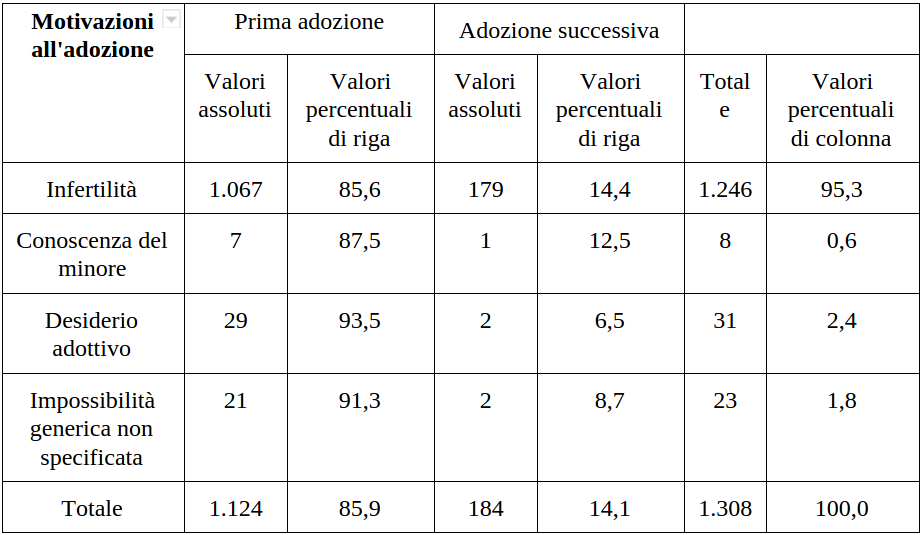
\includegraphics{./src/img/tavolacoppieadottive.png}
\caption{Commissione per le Adozioni Internazionali 2013, 14}
\end{figure}

\section{Allegato 2: Traccia
dell'intervista}\label{allegato-2-traccia-dellintervista}

\subsubsection*{Domande introduttive}\label{domande-introduttive}
\addcontentsline{toc}{subsubsection}{Domande introduttive}

Rispetto alla \textbf{composizione della famiglia}.

\begin{itemize}
\itemsep1pt\parskip0pt\parsep0pt
\item
  N° figli, nome, anni, paese d'origine, data di adozione
\end{itemize}

\subsubsection*{1° adozione}\label{adozione}
\addcontentsline{toc}{subsubsection}{1° adozione}

Focalizzazione sul primo percorso adottivo

\begin{itemize}
\item
  Adozione nazionale o internazionale? Se internazionale, con quale
  ente?
\item
  Preoccupazioni nell'attesa
\item
  Preoccupazioni dopo l'incontro
\item
  Problematiche post adozione. Le avevate prefigurate?
\end{itemize}

\subsubsection*{Tra 1° e 2° adozione}\label{tra-1-e-2-adozione}
\addcontentsline{toc}{subsubsection}{Tra 1° e 2° adozione}

\begin{itemize}
\item
  Motivazioni che vi hanno spinto ad intraprendere un secondo percorso
\item
  Dopo quanto tempo?
\item
  Siete stati consigliati nell'intraprenderlo?
\end{itemize}

(Parenti, Conoscenze di famiglie con seconde adozioni, supporto parere
psicologico)

\begin{itemize}
\itemsep1pt\parskip0pt\parsep0pt
\item
  Preoccupazioni rispetto ad un percorso adottivo non più di coppia ma
  ``di famiglia''?
\end{itemize}

(Reazioni fratellino? à GESTIONE EMOTIVA del primo figlio nel secondo
percorso adottivo, rivivere il percorso e il ``trauma'', il viaggio, il
tempo)

\begin{itemize}
\itemsep1pt\parskip0pt\parsep0pt
\item
  Coinvolgimento del primogenito e preparazione rispetto all'arrivo del
  secondogenito
\end{itemize}

\subsubsection*{2° adozione}\label{adozione-1}
\addcontentsline{toc}{subsubsection}{2° adozione}

Focalizzazione sul secondo percorso adottivo

\begin{itemize}
\itemsep1pt\parskip0pt\parsep0pt
\item
  Vissuto della seconda attesa. Stesse preoccupazioni?
\end{itemize}

(Sentimento di tutela del primogenito prevale sulla disponibilità
dell'accoglienza del secondo minore?

à aspetti tutelanti da preservare rispetto al primogenito es. maggiori o
minori disponibilità a pratiche sanitarie)

\begin{itemize}
\itemsep1pt\parskip0pt\parsep0pt
\item
  Difficoltà diverse rispetto al primo percorso? Aspettative.
\end{itemize}

(Aspettative positive e poca percezione delle eventuali difficoltà?
Salute, Incontro, Attaccamento)

\begin{itemize}
\item
  Complessità nella relazione tra i fratellini. Subito dopo l'incontro?
  Successivamente? Attualmente?
\item
  Altre problematiche post adozione? Le avevate prefigurate?
\item
  Quali sono stati nella vostra esperienza i fattori protettivi e i
  fattori critici nella relazione fraterna?
\end{itemize}

\chapter*{Bibliografia}\label{bibliografia}
\addcontentsline{toc}{chapter}{Bibliografia}

\setlength{\parindent}{0pt} \setlength{\parskip}{6pt plus 2pt minus 1pt}

AA.VV. (2003), \emph{Percorsi problematici dell'adozione internazionale.
Indagine sul fenomeno della ``restituzione''dei minori adottati da altri
paesi}. Firenze: Istituto degli Innocenti.

Cardano M., 2011, \emph{La ricerca qualitativa}, Il mulino, Bologna.

CIFA 2005, \emph{Bambini di carta\ldots{}bambini di carne}, Cifa Onlus,
Torino.

CAI (Commissione per le Adozioni Internazionali), 2013, \emph{Dati e
prospettive nelle Adozioni Internazionali. Rapporto sui fascicoli dal 1°
gennaio al 31 dicembre 2013}, Istituto degli Innocenti, Firenze.

\url{http://www.commissioneadozioni.it/media/143019/report_statistico_2013.pdf}

Visitato il 09/06/2015

Cavallo M., 2005, \emph{Figli cercasi. L'adozione internazionale:
istituzioni, leggi, casi}, Bruno Mondadori, Milano.

Corrias M., 2011, \emph{La seconda adozione}, in Italiaadozioni.

\url{http://www.italiaadozioni.it/?page_id=199}

Visitato il 09/06/2015

\emph{CRC}, \emph{Convenzione sui diritti dell'infanzia e
dell'adolescenza}, 20 novembre 1989, New York.

Cyrulnik B., Malaguti E., 2005, \emph{Costruire la resilienza. La
riorganizzazione positiva della vita e la creazione di legami
significativi}, Erickson edizioni, Trento.

De Rienzo E., Saccoccio C., Tonizzo F. e Viarengo G.,1999, \emph{Storie
di figli adottivi. L'adozione vista dai protagonisti}, Utet, Torino.

Franchetti M., Moro A., Macchi M., 2009, \emph{Fratelli d'adozione, le
seconde adozioni e le adozioni di fratelli, }in MINORIGIUSTIZIA
n°1/2009, pp.~273-282.

Galli J. e Viero F. (a cura di), 2001, \emph{Fallimenti adottivi.
Prevenzione e riparazione}, Armando editore, Roma.

Hague Adoption Convention, \emph{Convenzione sulla protezione dei minori
e sulla cooperazione in materia di adozione internazionale}, 29 maggio
1993, Aja.

Istituto degli Innocenti, 2013, \emph{Le famiglie e le informazioni
sullo stato di salute dei bambini adottati}, in \emph{I percorsi
dell'adozione internazionale: il punto di vista delle famiglie
l'esperienza delle famiglie. Indagine conoscitiva sulle coppie che hanno
adottato nel 2010}, Istituto degli Innocenti, Firenze, pp.43-47.

Lorenzini S., 2012, Famiglie per adozione. Le voci dei figli, ETS
editore, Pisa.

Lorenzini S., 2009, \emph{Famiglie adottive multiculturali: rapporti tra
fratelli e sorelle e ruoli genitoriali}, Rivista Italiana di Educazione
Familiare, n. 2 - 2009, pp.~23-33

Lorenzini S., Mancini M. P., 2007, \emph{Adozioni internazionali: un
nucleo interculturale di affetti, ma non sempre. Storie di adozioni
impossibili o fortemente problematiche}, Quaderno regionale n. 14,
Regione Emilia-Romagna, Bologna.

Lorenzini S., 2004, \emph{Adozione internazionale: genitori e figli tra
estraneità e familiarità}, Alberto Perdisa, Ozzano dell'Emilia (Bo);

Malaguti M., 2010, \emph{Valutare le competenze genitoriali
nell'adozione. Linee guida a confronto}, in S. Lorenzini (a cura di),
\emph{Focus Adozione nazionale e internazionale: alcune tematiche di un
universo familiare}, «Infanzia», 6, novembre-dicembre.

Rufo M., 2004, Fratelli e sorelle, Feltrinelli editore, Milano.

Scarpati M., 2012, \emph{I diritti dei bambini. Come aiutare noi e i
nostri figli a diventare adulti migliori}, Infinito edizioni, Modena.

Scialsi R., 2002, \emph{La gelosia tra fratelli}, Franco Angeli editore,
Milano.

Terrile P., Conti P., 2014, \emph{Figli che trasformano. La nascita
della relazione nella famiglia adottiva, }Franco Angeli editore, Milano.


\end{document}
